%--------------------------------------------------------------
% thesis.tex 
%--------------------------------------------------------------
% - template for the main file of Informatica@Unifi Thesis 
% - based on Classic Thesis Style Copyright (C) 2008 
%   Andr\'e Miede http://www.miede.de   
%--------------------------------------------------------------
\documentclass[openright,titlepage,oneside,fleqn,
	headinclude,12pt,a4paper,footinclude,makeidx]{scrbook}%twoside
%--------------------------------------------------------------
\usepackage[italian]{babel}
\usepackage[utf8]{inputenc} 
\usepackage[T1]{fontenc} 
\usepackage[square,numbers]{natbib} 
\usepackage[fleqn]{amsmath}
\usepackage{amssymb}
\usepackage{ellipsis}
\usepackage{listings}
\usepackage{subfig}
\usepackage[format=plain,labelformat=simple,labelsep=colon]{caption}
\usepackage{appendix}
\usepackage{siunitx}
\usepackage{lipsum}
\usepackage{dia-classicthesis-ldpkg}
\usepackage[eulerchapternumbers,linedheaders,subfig,beramono,eulermath,
parts,dottedtoc]{classicthesis}
\usepackage{imakeidx}
\usepackage{wrapfig}
\usepackage[italian,noabbrev]{cleveref}
%---------------------------------------------------------------
\newcommand{\myItalianTitle}{Titolo italiano.\xspace}
\newcommand{\myEnglishTitle}{Titolo inglese.\xspace}
\newcommand{\myDegree}{Master di I livello in Cybersecurity\xspace}
%\newcommand{\myCurriculum}{Resilient and secure cyberphysical systems\xspace}
\newcommand{\myName}{Marco Buracchi\xspace}
\newcommand{\myProf}{Tutor Accademico: Mario Rossi \\Tutor Aziendale: Carlo Bianchi\xspace}
\newcommand{\myFaculty}{Dipartimento di Ingegneria dell'Informazione\xspace}
\newcommand{\myUni}{\protect{Università di Pisa}\xspace}
\newcommand{\myLocation}{Pisa\xspace}
\newcommand{\myTime}{Anno Accademico 2018-2019\xspace}
\newcommand{\mycopyright}{
\includegraphics[width=1.5cm]{logo/cc.png} 
	\href{https://creativecommons.org/licenses/by-nc-sa/4.0/}{Creative
		Commons Attribution-NonCommercial-ShareAlike 4.0 International (CC BY-NC-SA 4.0)  }\xspace}

\newcommand{\disps}{dispositivo crittografico }
\newcommand{\dispp}{dispositivi crittografici }

\newcommand{\codice}[4]
	{\begin{center}
		\lstinputlisting[language={C},firstline={#1}, lastline={#2},caption={#3},label={#4}]{"C:/Users/mburacchi/Documents/analisiAPK/report/code/spark.c"}
	\end{center}}
\newcommand{\codspark}[3]{
	\begin{center}
		\lstinputlisting[language={C},firstline={#1},lastline={#2},firstnumber={#1},caption={[#3]}]{code/spark.c}
	\end{center}}

\newcommand{\arr}[2]{$\text{\texttt{#1}}\left[ \text{\texttt{#2}}\right]$}
\newcommand{\arrdoppio}[3]{$\text{\texttt{#1}}\left[ \text{\texttt{#2}} \left[\text{\texttt{#3}}\right]\right]$}

\newcommand{\kilobyte}{kB}
\newcommand{\megabyte}{MB}
\newcommand{\gigahertz}{GHz}

\newcommand{\tcal}{\mathbb{T}}
\newcommand{\talfa}{\mathbb{T}_{\alpha}}
\newcommand{\tbeta}{\mathbb{T}_{\beta}}

\newcommand{\myfloatalign}{\centering} 

\renewcommand{\lstlistingname}{Codice}% Listing -> Codice
%--------------------------------------------------------------
\newlength{\abcd} % for ab..z string length calculation
% how all the floats will be aligned
\setlength{\extrarowheight}{3pt} % increase table row height
\captionsetup{format=hang,font=small}
%--------------------------------------------------------------
% Layout setting
%--------------------------------------------------------------
\graphicspath{{img/}}
\usepackage{geometry}
\geometry{
	a4paper,
	ignoremp,
	bindingoffset = 1cm, 
	textwidth     = 13.5cm,
	textheight    = 21.5cm,
	lmargin       = 3.5cm, % left margin
	tmargin       = 4cm    % top margin 
}

\crefname{listing}{codice}{codici}

\lstset{ %
	basicstyle=\small\ttfamily, 		% the size of the fonts that are used for the code
	breaklines=true,                	% sets automatic line breaking
	captionpos=b,                   	% sets the caption-position to bottom
	commentstyle=\color{violet},   		% comment style
	frame=none,							% adds a frame around the code
	frameround=fttt,					% round corner (use f instead t to edge corner)
	keepspaces=true,                	% keeps spaces in text, useful for keeping indentation of code (possibly needs columns=flexible)
	keywordstyle=\color{blue},      	% keyword style
	language=C,               			% the language of the code
	numbers=left,                   	% where to put the line-numbers; possible values are (none, left, right)
	numbersep=5pt,                  	% how far the line-numbers are from the code
	numberstyle=\scriptsize\color{black}, % the style that is used for the line-numbers
	stepnumber=1,                   	% the step between two line-numbers. If it's 1, each line will be numbered
	stringstyle=\color{Brown},  		% string literal style
	tabsize=2                   		% sets default tabsize to 2 spaces
}

\makeindex[intoc]

%---------------------PARAMETERS-------------------------------
\begin{document}
\frenchspacing
\raggedbottom
\pagenumbering{roman}
\pagestyle{plain}

%---------------------FRONTMATTER------------------------------

%--------------------------------------------------------------
% titlepage.tex (use thesis.tex as main file)
%--------------------------------------------------------------
\begin{titlepage}
	\begin{center}
   	\large
      \hfill
      \vfill
      \begingroup
         
\includegraphics[scale=0.15]{logo/LOGO}\\
%\left 			\spacedallcaps{\myUni} \\ 
			\myFaculty \\
			\vspace{0.5cm}
			\myDegree \\ 
			Curriculum: \emph{\myCurriculum}\\
			\vspace{0.5cm}
         \vspace{0.5cm}    
         Tesi di Laurea Magistrale 
      \endgroup 
      \vfill 
      \begingroup
      	\color{Maroon}\spacedallcaps{\myItalianTitle} \\ $\ $\\
      	\spacedallcaps{\myEnglishTitle} \\ 	
	\bigskip
      \endgroup
      \spacedlowsmallcaps{\myName}
      \vfill 
      \vfill
      Relatore: Prof. \emph{\myProf}\\
      \vfill
      \vfill
      \myTime
      \vfill                      
	\end{center}        
\end{titlepage}   
%--------------------------------------------------------------
% back titlepage
%--------------------------------------------------------------
   \newpage
	\thispagestyle{empty}
	\hfill
	\vfill
	\noindent\myName: 
	\textit{\myItalianTitle,} 
	\myDegree, \mycopyright, \myUni, \myTime
%--------------------------------------------------------------
% back titlepage end
%--------------------------------------------------------------
\pagestyle{scrheadings}

%---------------------MAINMATTER-------------------------------

\pagenumbering{arabic}
\tableofcontents
\listoffigures
\lstlistoflistings

\begingroup
\let\clearpage\relax
\let\cleardoublepage\relax
\let\cleardoublepage\relax

\vspace*{8ex}

\listoftables
\endgroup 

\cleardoublepage
\thispagestyle{empty}

\begin{flushright}
\null\vspace{\stretch {1}}
\emph{"From camp to camp, through the foul womb of night,\\The hum of either army stilly sounds,\\That the fixed sentinels almost receive\\The secret whispers of each other’s watch."\\} 
\null\vspace{5mm}
\emph{"Da campo a campo, nel tetro grembo della notte,\\s’avverte appena il brusio di entrambe le armate,\\sicché le sentinelle appostate quasi possono udire\\i mormorii furtivi delle sentinelle nemiche" \break --- Enrico V, William Shakespear} \vspace{\stretch{2}}\null
\end{flushright}
\cleardoublepage

%-----------------CAPITOLI-------------------------------------

%\addcontentsline{toc}{chapter}{Introduzione}
\chapter*{Introduzione}
	\markboth{Introduzione}{}
	\lipsum
%	Il mondo moderno è ormai pervaso dalla \emph{crittografia}. Quotidianamente e spesso inconsapevolmente utilizziamo funzioni crittografiche per le normali operazioni della vita quotidiana. Controllare il conto sull'home-banking, scambiarsi messaggi tramite servizi di messaggistica o anche navigare in internet utilizzando il protocollo \acs{HTTPS} sono azioni che svolgiamo ormai con naturalezza. I sistemi moderni rendono trasparente all'utente l'utilizzo di tali tecnologie, ma ciò non vuol dire che esse non esistano.
%	
%	Una \emph{funzione crittografica}\index{Funzione crittografica} è un oggetto matematico astratto che, attraverso l'utilizzo di una chiave, trasforma un dato in input (plaintext) in una sua rappresentazione diversa (ciphertext) il più possibile non riconducibile al dato originale. Questa funzione deve poi essere implementata in un programma che girerà su un \emph{dispositivo crittografico} in un certo ambiente, presentando perciò caratteristiche fisiche peculiari. Esempi di \dispp potrebbero essere smartcard, chiavette \acs{USB}, chip dedicati montati su dispositivi general purpose (smartphone, notebook) o periferiche progettate e costruite apposta per effettuare questo unico compito.
%	
%	In passato si guardava ad un \disps semplicemente come una black-box che riceveva un plaintext e restituiva un ciphertext (encryption) e viceversa (decryption) come in \cref{fig:blackbox}. Gli attacchi erano basati sulla conoscenza del ciphertext (ciphertext-only attacks) o di alcune coppie di entrambi (known plaintext attacks). Con l'accesso al meccanismo di encryption o di decryption, anche solo temporaneo, si possono attuare anche altri due tipi di attacchi (rispettivamente chosen-plaintext e chosen-ciphertext)\cite{dispenseCS}.
%	
%	\begin{figure}
%		\begin{center}
%			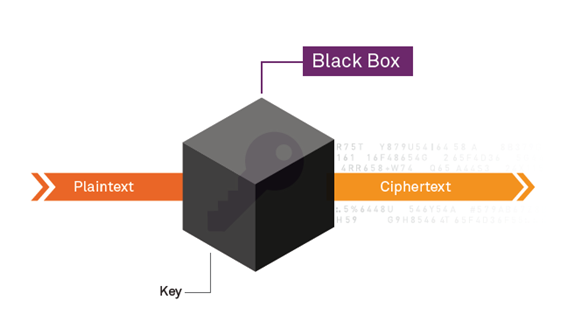
\includegraphics[width=.8\textwidth]{blackbox}
%			\caption{black-box encryption}
%			\label{fig:blackbox}
%		\end{center}
%	\end{figure}
%	
%	Al giorno d'oggi si è consapevoli del fatto che un \disps ha spesso altri input oltre al plaintext e altri output oltre al ciphertext. Gli input differenti dal plaintext possono essere le interazioni col mondo esterno come modifiche al voltaggio della corrente, condizioni atmosferiche particolari o sollecitazioni fisiche. Il nostro interesse sarà però focalizzato sulle informazioni (facilmente misurabili) che vengono lasciate trapelare dai dispositivi stessi oltre al ciphertext come ad esempio il tempo di esecuzione di un programma, le radiazioni emesse, suoni, luci e quant'altro chiamate \emph{side-channel informations}\index{Side-channel informations}.
%	 
%	 Il resto della tesi è organizzata nel seguente modo:
%	 \begin{itemize}
%	 	\item nel capitolo $1$, data l'eterogeneità della letteratura su questo argomento, abbiamo definito una classificazione dei side-channel attacks e abbiamo presentato una panoramica dello stato dell'arte.
%	 	\item nel capitolo $2$ abbiamo focalizzato la nostra attenzione sulla categoria dei \emph{timing attacks}, una particolare tipologia di side-channel attack basato sull'osservazione del tempo di esecuzione di un programma. Partendo da alcuni timing attack reali eseguiti su particolari funzioni crittografiche, abbiamo ottenuto una generalizzazione applicabile a qualunque attacco di questo tipo. Abbiamo anche implementato una piccola funzione crittografica ed effettuato una validazione sperimentale di questa nostra generalizzazione.
%	 	\item nel capitolo $3$ presentiamo i cache attacks, attacchi side-channel (prevalentemente di tipo timing) che colpiscono la memoria cache dei processori.
%	 	\item nel capitolo $4$ abbiamo presentato approfonditamente il progetto \emph{SPECTRE}, la principale famiglia di timing attacks sulle cache, che affligge tutti i recenti processori AMD, ARM e Intel.
%	 	\item nel capitolo $5$ descriviamo infine \ac{SPARK}, l'attacco da noi creato. Questo attacco, basato sui concetti del progetto SPECTRE, è in grado di ottenere dati protetti da password senza la conoscenza di quest'ultima.
%	 \end{itemize}    

%\chapter{Side-channel attacks}
	I \emph{side-channel attacks}\index{Side-channel attacks} sono metodi di crittoanalisi che sfruttano le side-channels informations insieme ad altre tecniche di analisi per recuperare la chiave utilizzata da un \disps\cite{standaert2010introduction}.
	
	\begin{figure}
		\begin{center}
			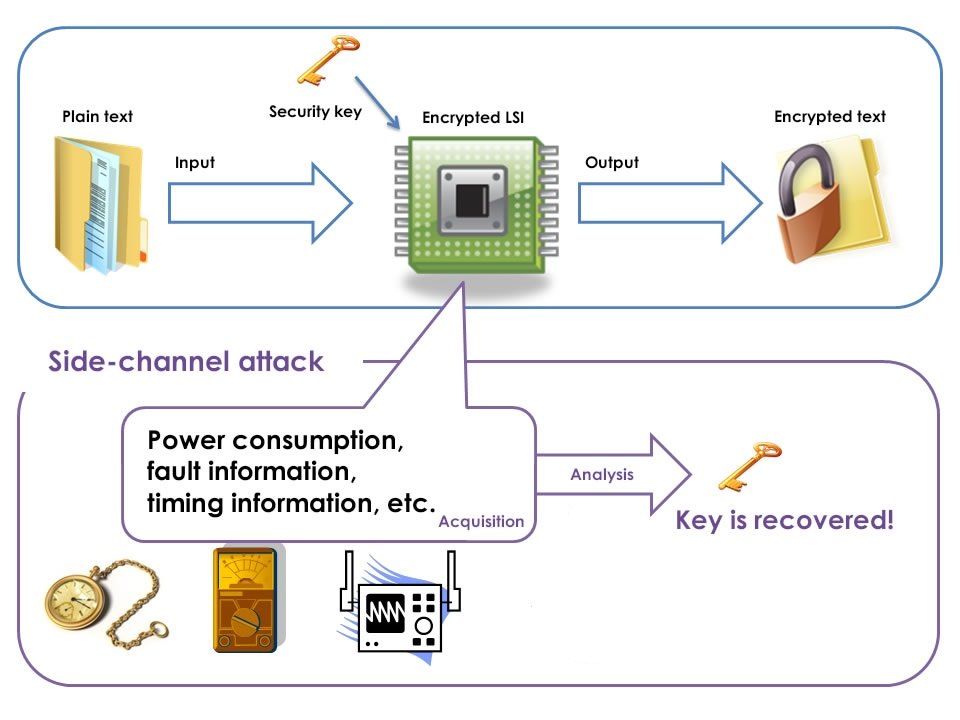
\includegraphics[scale=.4]{side-channel-attack_large}
			\caption{esempio di side-channel attack}
			\label{fig:attack}
		\end{center}
	\end{figure}
	
	Nella \cref{fig:attack} si può vedere una configurazione tipo di side-channel attack. La figura illustra il dispositivo che implementa la funzione crittografica con accanto alcune delle informazioni che è possibile estrapolare con tale tipologia d'attacco. La cosa fondamentale è che gli attacchi di questo tipo non vanno a colpire direttamente la funzione crittografica ma sfruttano le informazioni osservabili dell'ambiente circostante il dispositivo (parliamo quindi di grandezze fisiche).
	
	L'analisi di questi metodi ha acquisito notevole interesse poiché questo tipo di attacchi può essere montato velocemente e generalmente non richiede hardware particolare né costoso. Con pochi euro si possono ad esempio acquistare in comuni negozi di bricolage o elettronica apparecchi in grado di analizzare il consumo elettrico di un dispositivo. Con tali apparecchi è possibile montare in pochi secondi un attacco di tipo \emph{Simple Power Analysis}\cite{mangard2002simple} che verrà spiegato più avanti. 
	
	Il governo degli USA, nel suo "Orange book"\cite{latham1986department}, indica dei requisiti di sicurezza per i sistemi operativi. Questo documento introduce i primi standard per l'\emph{information leakage}. Purtroppo la letteratura specializzata è molto variegata e disomogenea, pertanto cercheremo innanzitutto di trovare un modo per classificare i vari tipi di attacchi in maniera tale da avere una visione più sistemistica del settore.
	
	\section{Classificazione degli attacchi}	
		Le caratteristiche che contraddistinguono ogni singolo attacco sono molteplici e differenti tra loro. In questa sezione si cercherà di raggruppare e definire quelle più importanti ed associabili alla maggior parte di essi.
	
		\subsection*{Tipi di canali}	
			Nel lavoro di \emph{Ge, Yarom, Cock} ed \emph{Heiser}\cite{ge2016survey} vengono fornite alcune definizioni che utilizzeremo nel prosieguo di questa tesi. La prima necessaria distinzione da fare è quella tra \emph{side-channel}\index{Side-channel} e \emph{covert-channel}\index{Covert channel}. Con i primi ci si riferisce ai canali che lasciano \emph{accidentalmente} filtrare informazioni sensibili (ad esempio una chiave crittografica) in una comunicazione tra due partecipanti fidati. I secondi sono invece canali creati e sfruttati dall'attaccante che lasciano passare \emph{deliberatamente} le informazioni, ad esempio i Trojan. In questo lavoro verranno trattati solamente i primi.
			
			L'altra differenza fondamentale è quella che riguarda i canali che possono essere divisi in canali di tipo \emph{storage}\index{Storage channel} e canali di tipo \emph{timing}\index{Timing channel}. I canali di tipo storage vengono sfruttati per ottenere qualcosa di direttamente visibile nel sistema (valore dei registri, valore di ritorno di una system call, ecc.). Quelli di tipo timing vengono sfruttati andando ad osservare variazioni del tempo di esecuzione di un programma (o di parti di esso).
			
		\subsection*{Tipi di attacco}		
			\emph{Standaert} nel suo lavoro \cite{standaert2010introduction} utilizza altre due dimensioni interessanti per classificare questi attacchi: l'\emph{invasività}\index{Invasività} e l'\emph{attività/passività}\index{Attività/passività}. 
			
			Si definisce \emph{invasivo} un attacco che richiede un disassemblamento del dispositivo attaccato per avere accesso diretto ai suoi componenti interni (wiretapping o sensori collegati direttamente all'hardware). Un attacco non invasivo, al contrario, sfrutta solamente le informazioni disponibili esternamente (quasi sempre involontarie) come il tempo d'esecuzione o l'energia consumata.
			
			Si definisce \emph{attivo} un attacco che cerca di interferire con il corretto funzionamento del dispositivo (fault-injection)\cite{giraud2004dfa,karri2001fault}, mentre un attacco passivo si limita ad osservare il comportamento del dispositivo durante il suo lavoro senza disturbarlo. 
			
		\subsection*{Grandezza fisica osservata}		
			Una caratteristica molto importante di questi attacchi è sicuramente la grandezza fisica che viene osservata per montare l'attacco. Teoricamente, qualunque grandezza fisica misurabile può essere sfruttata, ma alcune sono più facilmente attaccabili rispetto ad altre. 
			
			Tra le varie grandezze fisiche, tempo e consumo energetico sono quelle più comunemente utilizzate, ma non certo le uniche. \emph{Genkin, Shamir e Tromer} nel loro lavoro \cite{genkin2014rsa} vanno ad ascoltare i rumori prodotti dal processore. \emph{Ferrigno} e \emph{Hlavac}\cite{ferrigno2008aes} osservano la luce (qualche fotone) emessa dai transistor nel passaggio di stato da $0$ a $1$. \emph{Martinasek, Zeman} e \emph{Trasy}\cite{martinasek2012simple} sfruttano i campi elettromagnetici creati dai chip. \emph{Murdoch}, attraverso le variazioni delle frequenze del clock, ricava informazioni sulla temperatura ambientale e cerca di localizzare geograficamente il dispositivo della vittima.
			
			Questo elenco assolutamente non esaustivo delle tecniche utilizzate può far capire quanto variegato ed eterogeneo (nonché in continua evoluzione) sia questo settore.
			
		\subsection*{Hardware attaccato}		
			Gli attacchi possono essere suddivisi anche in base alla componente hardware che viene attaccata. Anche in questo caso ci sono componenti più attaccati (ed attaccabili) di altri (cache e processori), ma non mancano esempi di attacchi a monitor\cite{van1985electromagn}, tastiere\cite{asonov2004keyboard} o stampanti\cite{backes2010acoustic}.
			
		\subsection*{Algoritmo attaccato}		
			È infine possibile classificare gli attacchi a seconda dell'algoritmo crittografico attaccato. In questo caso i due maggiori algoritmi attaccati sono senza dubbio \ac{AES}\cite{standard2001announcing} ed RSA\cite{rivest1978method} nelle loro implementazioni più comuni. Altri algoritmi attaccati sono El-Gamal\cite{elgamal1985public} e le curve ellittiche\cite{koblitz1987elliptic,miller1985use}.
			\begin{table}[]
				\scriptsize
				\centering
				\begin{tabular}{|c|c|c|c|c|c|c|c|} \hline
					Fonte						& Grandezza					& Componente	& Algoritmo			& Invasivo	& Attivo	& Canale	& Anno		\\ \hline \hline
					\cite{genkin2014rsa}		& Suono						& CPU			& RSA				& No		& No		& -			& $2014$	\\ \hline
					\cite{ferrigno2008aes}		& Luce						& Transistor	& AES				& Sì		& No		& -			& $2008$	\\ \hline
					\cite{van1985electromagn}	& Campo elettromagnetico	& Monitor    	& -					& No		& No		& -			& $1985$	\\ \hline
					\cite{kocher2018spectre}	& Tempo						& Cache			& RSA				& No		& No		& Timing	& $2018$	\\ \hline
					\cite{giraud2004dfa}		& -							& -				& AES				& No		& Sì		& Storage	& $2004$	\\ \hline
					\cite{mangard2002simple}	& Consumo elettrico			& Smartcard		& AES				& No		& No		& -			& $2002$	\\ \hline
					\cite{asonov2004keyboard}	& Suono						& Tastiere		& -					& No		& No		& -			& $2004$	\\ \hline
					\cite{zhou2018efficient}	& Tempo						& Cache			& OpenSSL			& No		& No		& Timing	& $2018$	\\ \hline
					\cite{martinasek2012simple}	& Campo elettromagnetico	& Chip			& AES				& No		& No		& -			& $2012$	\\ \hline
					\cite{yarom2014flush+}		& Tempo						& Cache			& RSA				& No		& No		& Timing	& $2014$	\\ \hline
					\cite{karri2001fault}		& -							& -				& AES				& No		& Sì		& Storage	& $2001$	\\ \hline
					\cite{backes2010acoustic}	& Suono						& Stampanti		& -					& No		& No		& -			& $2010$	\\ \hline
					\cite{lipp2016armageddon}	& Tempo						& Cache			& AES				& No		& No		& Timing	& $2016$	\\ \hline
					\cite{murdoch2006hot}		& Temperatura				& Clock			& -					& No		& No		& -			& $2006$	\\ \hline
					\cite{genkin2018drive}		& Tempo						& Browser		& Curve ellittiche	& No		& No		& Timing	& $2018$	\\ \hline
				\end{tabular}
				\caption{classificazione dei principali attacchi conosciuti}
				\label{tab:attacchi}
			\end{table}
			Nella \cref{tab:attacchi} sono classificati i principali attacchi conosciuti usando i criteri ora esposti.
			
			Passiamo adesso ad una breve panoramica sui maggiori attacchi per ogni tipo di grandezza fisica sfruttata per l'attacco. Si ricorda che gli attacchi basati sul tempo, categoria nella quale ricadono la maggior parte degli attacchi eseguiti contro le cache, verranno approfonditi nel prossimo capitolo.
			
	\section{Attacchi basati sul campo elettromagnetico}\index{Electromagnetic attacks}
		Fin dalla metà del $1900$, il governo degli Stati Uniti d'America era a conoscenza del fatto che i computer producessero "emanazioni compromettenti" e che queste potessero essere rilevate ed utilizzate. I ricercatori dell'esercito dimostrarono che era possibile catturare queste emanazioni a distanza e rivelare le informazioni (classificate) ad esse associate. In relazione a questo problema fu attivato il progetto \ac{TEMPEST}.\index{TEMPEST}
		
		TEMPEST è uno standard creato dal \ac{NCSCD4} ed i requisiti richiesti alle periferiche TEMPEST-compliant sono specificati nel documento riservato NACSIM5100A. Anche la \ac{NATO} possiede uno standard di protezione simile chiamato SDIP-$27$.
		
		Nel suo libro\cite{wright1987spycatcher}, \emph{Peter Wright}, ex ricercatore dei servizi segreti inglesi (MI$5$), rivela l'origine degli attacchi di tipo TEMPEST su macchine cifranti. I principali enti governativi utilizzano, sui sistemi ritenuti sensibili, speciali protezioni come scudi metallici molto costosi su singoli dispositivi, stanze o interi edifici\cite{herndon1990electromagnetic}.
		
		Il primo documento pubblico riguardante le minacce alla sicurezza prodotte dalle emanazioni dei computer (primo esempio pubblico di side-channel attack) risale al $1985$ ed è opera di \emph{Wim van Eck}\cite{van1985electromagn}. Nel suo lavoro dimostrò come fosse possibile ricostruire l'immagine prodotta da un monitor attraverso l'analisi a distanza del campo elettromagnetico emesso, riproducendola su un altro schermo. La comunità scientifica specializzata nella sicurezza era già a conoscenza di questo fenomeno, che veniva però ritenuto di poco interesse perché si pensava che servissero attrezzature molto costose, disponibili soltanto per uso militare. Van Eck li smentì ricostruendo l'immagine di un monitor posto a centinaia di metri di distanza usando solamente un televisore modificato con quindici dollari di accessori (al cambio attuale corrisponderebbero a meno di quaranta euro).
		
		Nel corso degli anni tali tipi di attacco si sono evoluti andando a colpire schermi piatti\cite{kuhn2006eavesdropping}, chip\cite{martinasek2012simple}, tastiere\cite{vuagnoux2009compromising} e in generale qualunque dispositivo contenente componenti elettronici in grado quindi di produrre onde elettromagnetiche.
			
	\section{Attacchi basati sul suono}\index{Acoustic attacks}
		L'analisi dei suoni prodotti da dispositivi meccanici, specialmente in campo militare, risale a molto indietro quando si riusciva a distinguere un aereo o un sommergibile a seconda del rumore prodotto.
	
		Anche i dispositivi elettronici, in generale, emettono un grande numero di rumori diversi. Se ad esempio pensiamo ad un computer portatile, alcune informazioni banali che possiamo ricavare dai suoni emessi sono l'attività dell'Hard Disk che ci suggerisce un utilizzo della memoria oppure l'accendersi di una ventola che ci suggerisce un intenso utilizzo della CPU. Questo tipo di informazioni sono però troppo generiche, specialmente in un dispositivo general purpose che esegue molti processi diversi parallelamente.
	
		Per approfondire il livello di informazione ricevuto, le strade più percorse sono due: aumentare la sensibilità dell'ascoltatore cercando di trovare differenze tra rumori che sembrano uguali o ascoltare rumori più particolari.
	
		\subsection{Differenziazione dei rumori}	
			Uno degli esempi più importanti di questo tipo di attacco è quello eseguito sulle stampanti a matrice di aghi nel $2010$\cite{backes2010acoustic}. Il fatto che questo tipo di stampanti non venga pressoché più utilizzato dal privato cittadino, non faccia supporre che l'attacco sia anacronistico. La scelta di attaccare proprio questa categoria di stampanti è infatti dovuta al fatto che in quell'anno circa il $60\%$ dei medici in Germania e il $30\%$ delle banche le utilizzavano ancora. Alcuni stati europei richiedono per legge l'utilizzo di stampanti a matrici di aghi per la prescrizione di particolari medicine\cite{bernatzky2011schmerzbehandlung}.
			
			\begin{figure}
				\begin{center}
					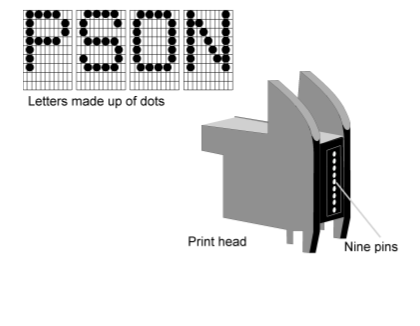
\includegraphics[scale=.5]{printMatrix}
					\caption{modalità di stampa di una stampante ad aghi}
					\label{fig:matrixHead}
				\end{center}
			\end{figure}
			
			Come si vede in \cref{fig:matrixHead}, una stampante ad aghi scompone ogni lettera in colonne di punti ed utilizza gli aghi necessari per incidere la traccia corretta sulla carta. Lo studio dimostra come sia possibile addestrare una rete neurale per riconoscere il rumore emesso ad ogni singolo passo che cambia in base a quanti e quali aghi vengono utilizzati. Tale rete neurale riconosce il $72\%$ delle parole stampate senza alcuna ulteriore assunzione ed arriva al $95\%$ se si assume una conoscenza del contesto.
			
			L'idea di base è la stessa utilizzata anche in \cite{asonov2004keyboard} nel $2004$ per riconoscere i rumori prodotti dai tasti premuti su di una tastiera.
		
		\subsection{Cogliere rumori impercettibili}	
			In questa seconda categoria uno dei principali rappresentati è sicuramente l'attacco\cite{genkin2014rsa} del $2014$ portato contro il circuito di regolazione del voltaggio dei computer. Tale circuito è composto da bobine e condensatori che vibrano nel tentativo di fornire un voltaggio costante alla CPU.
			
			Eseguire ad esempio RSA con chiavi differenti produce pattern di esecuzione di operazioni della CPU diversi che portano all'utilizzo di quantità di energia elettrica differente. Il regolatore di voltaggio reagisce di conseguenza causando fluttuazioni di elettricità che provocano vibrazioni meccaniche nei componenti elettronici e queste vibrazioni vengono trasmesse attraverso l'aria come onde sonore. Il riconoscimento di questi pattern differenti permette agli autori di recuperare la chiave RSA utilizzata.
			
			La particolarità interessante di questo attacco è che non richiede un'attrezzatura complessa ed avanzata. Il risultato migliore viene ovviamente ottenuto con un microfono direzionale professionale posizionato ad una distanza di quattro metri dal computer attaccato, ma lo stesso risultato viene ottenuto anche con l'utilizzo di un semplice smartphone posto a 30 cm dallo stesso computer.
			
	\section{Attacchi basati sulla luce}\index{Optical attacks}
		Le emissioni ottiche sono un'altra possibile fonte di informazioni. Alcune di queste, le più banali, possono ad esempio essere ricavate dalla semplice osservazione dei \acs{LED} presenti su ogni dispositivo che informano sullo stato del dispositivo stesso. Si può capire se un dispositivo è acceso o spento, se sta eseguendo computazioni o è inattivo, se sta recuperando informazioni in memoria o se sta utilizzando la connessione Wi-Fi. Simili informazioni sono tutte facilmente osservabili, ma, nella maggior parte dei casi, poco utili.
		
		Per ottenere informazioni più significative occorre dotarsi di strumenti di rilevazione più avanzati e utilizzare metodi più "invasivi".
		
		\emph{Ferrigno} nel suo lavoro\cite{ferrigno2008aes} si basa sulla seguente idea: ogni volta che un transistor presente su un circuito integrato cambia il proprio stato (passa da $0$ a $1$ ad esempio) emette qualche fotone. Grazie all'utilizzo di \emph{Optica}, un dispositivo presente nei laboratori del \ac{CNES} il cui costo è dell'ordine del milione di euro, si riescono a rilevare questi fotoni e a capire il passaggio di stato del singolo transistor tramite la tecnica chiamata \ac{PICA}\cite{tsang2000picosecond}.
		
		I principali problemi che presenta questo attacco sono il costo dello strumento di rilevazione e l'invasività (bisogna infatti esporre completamente il circuito integrato), ma riesce a captare qualunque informazione si voglia a patto di conoscere il programma che sta girando in quel momento.
				
		La necessità di conoscere il programma, insieme a quella di sincronizzare Optica col codice che sta eseguendo il dispositivo, costuituisce un ulteriore problema. Una soluzione come la randomizzazione delle operazioni utilizzata nei processori moderni rende questo attacco molto più difficile da realizzare.
			
	\section{Attacchi basati sul consumo elettrico}\index{Power analysis attacks}
		Questo tipo di attacchi si basa sull'analisi del consumo energetico di un \disps mentre esegue una encryption o una decryption. Gli attacchi "classici" di questo tipo sono la \ac{SPA} e la \ac{DPA} entrambe introdotte da \emph{Kocher}\cite{kocher2011introduction}.
		
		\subsection{Simple Power Analysis}\index{Simple Power Analysis}
		Nella \ac{SPA} l'attaccante osserva il consumo energetico istantaneo del dispositivo. Questo consumo è direttamente dipendente dalle istruzioni eseguite dal microprocessore. Funzioni complesse come il \ac{DES} o RSA possono essere identificate grazie alla grande differenza di operazioni svolte dal processore nelle varie parti che compongono questi algoritmi. 
		
		Visto che la \ac{SPA} riesce a rivelare la sequenza di istruzioni eseguita, può essere usata per attaccare implementazioni di funzioni crittografiche che richiedono l'esecuzione di precisi path di operazioni a seconda dei dati forniti in input. Le permutazioni di \ac{DES} come le moltiplicazioni o le esponenziazioni di RSA sono vittime tipiche di questi attacchi.
		
		\begin{figure}
			\begin{center}
				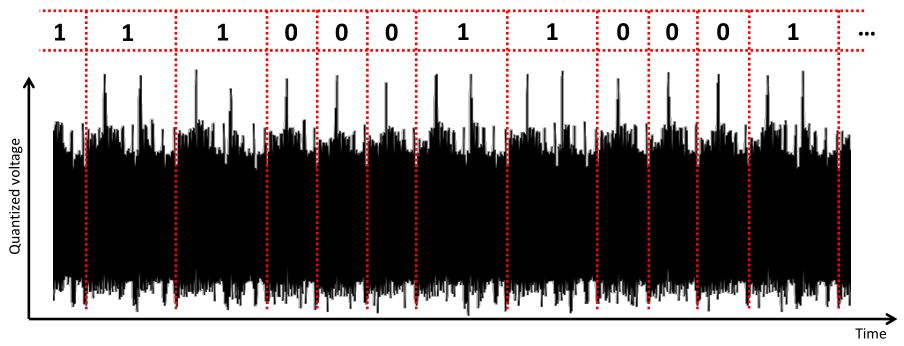
\includegraphics[scale=.5]{powerRSA}
				\caption{SPA contro RSA}
				\label{fig:RSAPower}
			\end{center}
		\end{figure}
	
		Prendiamo ad esempio RSA: le operazioni che esegue ad ogni passo di encryption/decryption possono essere tre (square, reduce e multiply) e dipendono dalla chiave. Questa viene scandita bit a bit e, se l'i-esimo bit è un $1$, RSA esegue la sequenza square-reduce-multiply-reduce, altrimenti esegue solamente la sequenza square-reduce. \`{E} possibile riconoscere questi pattern dall'analisi del consumo energetico, come si può vedere in \cref{fig:RSAPower}. 
		
		\subsection{Differential Power Analysis}\index{Differential Power Analysis}
			La \ac{DPA} è un attacco più sofisticato della \ac{SPA} perché aggiunge all'analisi istantanea del consumo anche un'analisi statistica. Per questo motivo è più potente e più difficile da prevenire (ma è anche più costoso in termini di tempo).
			
			Generalmente un attacco \ac{DPA} si divide in una fase di raccolta dei dati e in una fase di analisi statistica degli stessi. L'utilizzo di tecniche statistiche elaborate, da una parte "filtra" i dati dalle possibili sorgenti di rumore e dall'altra può permettere di estrarre maggiori informazioni rispetto alla semplice esecuzione delle singole operazioni. 
	
	\section{Attacchi basati sulla temperatura}\index{Temperature attacks}
		Esistono numerosi esempi in letteratura di attacchi basati sulla temperatura \cite{brouchier2009temperature,brouchier2009thermocommunication,skorobogatov2002low}, ma la maggior parte delle pubblicazioni in merito si limita a confermare l'esistenza del metodo e la possibilità di sfruttare tale canale, senza ulteriori approfondimenti.
		In particolare, in \cite{bar2006sorcerer}, si afferma che attacchi di questo tipo su smart-card sono "\emph{never documented in the open literature to the author’s knowledge}".
			
		L'unica pubblicazione in cui viene effettivamente eseguito un attacco basato sulla temperatura contro un algoritmo crittografico è quello di \emph{Brouchier et al.}\cite{brouchier2009temperature}, che dimostra come una ventola di raffreddamento può portare indirettamente informazioni sui dati processati analizzando la necessità di dissipazione del calore da parte del computer.
		
		Un altro lavoro interessante è quello di \emph{Murdoch}\cite{murdoch2006hot} nel quale si sfrutta la seguente idea: il tempo misurato dal clock di un computer non è costante, ma tende a discostarsi dal tempo "reale" (ad esempio quello fornito dal \acs{GPS}) con un certo tasso che può dipendere anche dalla temperatura\cite{vig1992introduction}. Attraverso la richiesta di timestamps alla vittima è possibile calcolare questo tasso, capire il relativo carico di lavoro e deanonimizzare la vittima da una rete \acs{TOR}.
		
	\section{Attacchi fault-based}\index{Fault-based attacks}
		Gli attacchi basati sui fault si ottengono introducendo intenzionalmente degli errori nella normale esecuzione di un algoritmo crittografico. Tale esecuzione modificata può far trapelare informazioni che possono essere utilizzate per recuperare la chiave. In generale gli attacchi fault-based si dividono in quattro categorie\cite{patranabis2018fault} descritte qui sotto.
		
		\subsection*{\ac{DFA}}
			La \ac{DFA}\index{Differential fault analysis} è una tecnica nella quale l'attaccante inserisce un errore durante la computazione in un fissato punto spazio-temporale dell'algoritmo e successivamente analizza le differenze tra il ciphertext esatto e quello errato per recuperare la chiave segreta. Tecniche di \ac{DFA} sono state applicate ai principali algoritmi crittografici, soprattutto su \ac{AES}-$128$. Allo stato dell'arte, tale attacco permette di recuperare l'intera chiave a $128$ bit di \ac{AES} con l'inserimento di un singolo fault\cite{tunstall2011differential}.
			
		\subsection*{\ac{FSA}}
			La \ac{FSA}\index{Fault sensitivity analysis} è stata introdotta da \emph{Li et al.}\cite{li2010fault} ed è una tecnica che non utilizza direttamente i ciphertext ottenuti tramite una computazione in presenza di fault. Nel loro lavoro gli autori cercano di trovare delle condizioni critiche che fanno assumere al ciphertext alcune caratteristiche riconoscibili (ad esempio la frequenza di clock al momento dell'esecuzione dell'istruzione difettosa) chiamate \emph{fault sensitivity}. La \ac{FSA} sfrutta poi le relazioni tra queste caratteristiche e i dati processati per recuperare informazioni segrete dal \disps.
			
		\subsection*{\ac{DFIA}}
			La \ac{DFIA}\index{Differential fault intensity analysis} è stata introdotta da \emph{Ghalaty et al.}\cite{ghalaty2014differential} ed è una classe di attacchi che combina tecniche di \ac{DPA} con tecniche di fault analysis per il recupero di chiavi\cite{fuhr2013fault}. Gli autori osservano che la maggior parte dei fault restituiscono byte con un numero di bit errati non sempre uguale (generalmente da 1 a 3) e che questa informazione può essere sfruttata per rivelare la chiave segreta attraverso un test di verifica d'ipotesi. Data la sua natura statistica, la \ac{DFIA} ha bisogno di un gran numero di modelli di fault, ma è comunque una minaccia importante verso molti cifrari a blocchi.
			
		\subsection*{\ac{SEA} e \ac{DBA}}
			\index{Safe-Error attacks}\index{Differential behavior analysis}Questa ultima categoria di attacchi mira a dedurre dal comportamento di un \disps se un fault che ha portato ad una computazione scorretta è avvenuto durante una operazione di encryption oppure no\cite{robisson2007differential}. Questa categoria si sta sviluppando nella direzione della \ac{FBA} (tecnica introdotta da \emph{Li et al.} in \cite{li2014yet}). Questi attacchi osservano solamente il comportamento del \disps durante l'iniezione dei fault, pertanto non è richiesta la conoscenza del valore del ciphertext.
			
	\section{Possibili contromisure}	
		Le possibili contromisure a questi attacchi sono molteplici, sia fisiche che algoritmiche.
		
		Le soluzioni fisiche(\cite{anderson1996tamper,shamir2000protecting,tuyls2006read,tiri2002dynamic}) sono quelle che cercano di evitare il rilascio di informazioni nell'ambiente circostante il dispositivo. Insonorizzazione, schermature e utilizzo di circuiti \emph{dummy} che eseguono istruzioni fasulle per uniformare il consumo elettrico sono tutti esempi di contromisure fisiche sicuramente funzionanti, ma che richiedono sforzi di progettazione maggiore con conseguente aumento dei costi di produzione.
		
		Le soluzioni che stanno andando per la maggiore sono quelle software, come ad esempio la randomizzazione dell'input\cite{boscher2012randomized}. Se parliamo di RSA possiamo pensare ad esempio di modificare l'esponente o il modulo ad ogni iterazione sommandoci un valore casuale che poi verrà sottratto in maniera opportuna. In questo modo le analisi dirette delle operazioni vengono "mascherate" ed anche le possibilità di correlazioni statistiche vengono (quasi) annullate.
		
		Questo tipo di soluzioni possono risolvere il problema, ma richiedono cambiamenti nel design degli algoritmi e dei protocolli che rischiano di rendere il prodotto incompatibile con standard o specifiche pubbliche.
%\chapter{Timing attacks}
\index{Timing attacks}Come anticipato nel capitolo precedente, approfondiremo adesso la tipologia di attacchi basati sul tempo (timing attacks). 

I timing attacks si basano sulla misurazione del tempo necessario ad un dispositivo per effettuare un'operazione. Tali rivelazioni possono portare all'esposizione di alcune informazioni sull'operazione stessa o sui dati da essa manipolati. Questo accade perché molto spesso la durata di un'operazione dipende dagli input che vengono forniti dall'esterno.

Le istruzioni che prestano maggiormente il fianco a questo tipo di attacchi sono le istruzioni di branch e i condizionali.

\begin{center}
	\lstinputlisting[language={Java}, caption={esempio di funzione vulnerabile ad un timing attack}, label={list:timingBase}, frame={none},basicstyle={\small\ttfamily}]{code/timingBase.txt}
\end{center}

Ad esempio, un programma implementato con il \cref{list:timingBase}, se fatto girare con la stringa "\texttt{passwordToBeStolen}" impiegherà un tempo maggiore rispetto allo stesso programma fatto girare con la stringa "\texttt{foo}". Nel primo caso infatti verrà scansionata tutta la stringa, mentre nel secondo caso si interromperà immediatamente. Questa informazione può essere utilizzata dall'attaccante che, procedendo per tentativi, può arrivare a ricavare la stringa esatta.

Questo esempio banale non deve portare a pensare che le caratteristiche temporali di una certa operazione rivelino solamente informazioni su una piccola parte di un intero sistema crittografico. Come dimostrato da \emph{Kocher} in \cite{kocher1996timing} esistono attacchi che, solamente sfruttando misurazioni di tempi di esecuzione di particolari operazioni, riescono a scoprire l'intera chiave in implementazioni diverse di algoritmi crittografici complessi come \emph{RSA}, \ac{DH} o \ac{DSS}.

Per ottenere tali risultati, le misurazioni dei tempi vengono analizzate con un modello statistico che scopre la chiave con un certo intervallo di confidenza, progredendo di un bit alla volta. Il modello deve essere in grado di controllare la correlazione tra le varie misurazioni e stabilire di conseguenza se il successivo bit della chiave debba essere $0$ oppure $1$.

	\section{Attacchi reali}
	
	Analizziamo tre attacchi reali presi proprio dall'articolo di \emph{Kocher}.
	
		\subsection{Esponenziazione modulare}
		Un'operazione comune utilizzata sia da \ac{DH} che da RSA è il calcolo di $$R = y^{x} \ mod \ n.$$ In questa operazione, $n$ è pubblico e $y$ può essere trovato tramite una qualche intercettazione di messaggi da parte dell'attaccante. Lo scopo finale dell'attacco sarà quello di trovare $x$, la chiave segreta.
		
		Per questo attacco, fissata una $x$, la vittima deve calcolare $y^{x} \ mod \ n$ per diversi valori di $y$, e l'attaccante deve conoscere $y$, $n$ e il tempo necessario al calcolo.
		Analizzando statisticamente queste misurazioni, si riesce a risalire all'intera chiave segreta.
		
		Le informazioni necessarie e le misurazioni temporali posso essere ottenute passivamente tramite qualche forma di intercettazione (ad esempio creando un \emph{man-in-the-middle}) sul protocollo di comunicazione fornito dalla vittima. L'attaccante a questo punto conosce il messaggio ricevuto dalla vittima e misura il tempo che essa impiega per rispondere con il risultato utilizzando vari $y$.
		
		Questo attacco può essere adattato ad ogni implementazione di questa operazione, all'unica condizione che non si tratti di una delle varianti che lavora in tempo costante.
		
		\subsection{Moltiplicazione di Montgomery e Chinese Remainder Theorem}
		In un'operazione di moltiplicazione modulo $n$, il passo di riduzione modulare è il principale responsabile delle variazioni nel tempo di esecuzione. La moltiplicazione di \emph{Montgomery}\cite{montgomery1985modular} elimina il passo di riduzione modulo $n$ riducendo il tempo totale dell'operazione e, di conseguenza, anche le variazioni associate.
		
		Per ottimizzare le operazioni che utilizzano la chiave privata di RSA viene utilizzato anche il \ac{CRT}. Se il messaggio da cifrare è $y$, utilizzando il \ac{CRT} si calcolano inizialmente $(y \ mod \ p)$ e $(y \ mod \ q)$. Queste due operazioni iniziali sono la parte dell'algoritmo vulnerabile ai timing attacks. Il più semplice di questi attacchi sceglie un valore $y$ che si suppone vicino a $p$ o $q$. Successivamente utilizza i tempi di esecuzione per capire se $y$ sia più grande o più piccolo di $p$ (o di $q$). Se $y < p$, il calcolo di $y \ mod \ p$ non esegue alcuna operazione, mentre se $y \geq p$, sarà necessario sottrarre $p$ da $y$ almeno una volta aumentando il tempo di esecuzione.
		
		Le caratteristiche esatte dell'attacco dipendono dall'implementazione dell'algoritmo attaccato.
		
		\subsection{Digital Signature Algorithm}
		Il \ac{DSA} è uno standard \ac{FIPS} per la firma digitale proposto dal \ac{NIST} nell'agosto del 1991 per essere impiegato nel \ac{DSS}, e adottato definitivamente nel 1993. Le sue specifiche sono contenute nel documento \ac{FIPS}-186\cite{kravitz1993digital}.
		
		Il \ac{DSS} calcola $s = (k^{-1}(H(m) + x \cdot r)) \ mod \ q$ dove $r$ e $q$ sono noti all'attaccante, $k^{-1}$ è precalcolato, $H(m)$ è l'hash del messaggio e $x$ è la chiave privata.
		
		Se l'operazione di riduzione modulo $q$ non è stata implementata per funzionare a tempo costante, esiste una correlazione tra il tempo totale di computazione e quello necessario per eseguire $(x \cdot r \ mod \ q)$. L'attaccante può quindi calcolare tale tempo in modi simili a quelli visti in precedenza, e scoprire la chiave segreta $x$.
		
	\section{Generalizzazione}
	Abbiamo appena illustrato tre casi concreti di timing attacks contro specifici algoritmi crittografici. Partendo da queste basi, abbiamo cercato una generalizzazione applicabile alla maggior parte degli attacchi di questo tipo.
	
	Abbiamo notato che tutte le informazioni che vengono ricavate sono connesse alle variazioni del tempo di esecuzione, e dipendono in qualche modo dal segreto che l'attaccante vuole scoprire.
	
	Abbiamo supposto che l'attaccante prenda di mira una specifica istruzione \texttt{if} nel codice, come ad esempio \texttt{if p(h) then c} dove \texttt{p(.)} è un predicato con valore $0/1$ su \texttt{h}, in un contesto \texttt{B[.]}. In questo caso, l'intero programma sarebbe \texttt{B[if p(h) then c]}.
	
	Abbiamo assunto che il tempo di esecuzione dipenda da alcuni input forniti al programma che modificano l'esecuzione di \texttt{c}. Considerando i.i.d questi input e fissando il segreto \texttt{h}, abbiamo definito il tempo di esecuzione dell'intero programma come una variabile aleatoria $\tcal$ che può essere divisa in \begin{equation} \label{eq:1}
		\tcal = \talfa + \text{\texttt{p(h)}}\cdot \tbeta
	\end{equation} 
	dove $\talfa$ è il tempo di esecuzione dovuto a \texttt{B} e $\tbeta$ quello dovuto a \texttt{c} in una completa esecuzione di \texttt{B[c]}.
	
	Lo scopo dell'attaccante è quello di scoprire il valore di \texttt{p(h)} (che potrebbe rappresentare l'i-esimo bit della chiave) attraverso misurazioni del tempo di esecuzione dell'intero programma.
	
	A questo proposito è immediato vedere che $$var(\tcal)=\left\{\begin{array}{ll}
	var(\talfa) & \mathrm{s}\mathrm{e}\ \text{\texttt{p(h)}} = 0\\
	var(\talfa)+var(\tbeta)+2\cdot cov (\talfa,\tbeta) & \mathrm{s}\mathrm{e}\ \text{\texttt{p(h)}} = 1
	\end{array}\right.$$ 
	
	da cui ricaviamo che $$var(\tcal) > var(\talfa) \Leftrightarrow \text{\texttt{p(h)}} = 1$$ 
	
	a condizione che 
	\begin{equation} \label{eq:2}
		var(\tbeta) > 2 \cdot |cov(\talfa,\tbeta)|.
	\end{equation}
		
	Questa formulazione però non è sufficiente per l'attaccante visto che, sebbene possa stimare facilmente $var(\tcal)$, non ha modo di stimare $var(\talfa)$ a meno che non sia in grado di eseguire \texttt{B} in isolamento (ipotesi troppo forte e poco realistica). Abbiamo pensato che l'attaccante potrebbe però simulare \texttt{c}, calcolare $\tbeta$ e confrontare $var(\tcal - \tbeta)$ con $var(\tcal)$. 
	
	Il risultato che abbiamo ottenuto è stato dimostrare che $$var(\tcal - \tbeta) < var(\tcal) \Leftrightarrow \text{\texttt{p(h)} = 1}.$$ Questi sono tutti valori calcolabili (o perlomeno stimabili).\\
	
	\subsection{Dimostrazione} 
		Dimostrazione $\Leftarrow$:\\
		Se $\text{\texttt{p(h)}} = 1$, allora dall'\cref{eq:1} $$\tcal = \talfa + \tbeta \Rightarrow \tcal - \tbeta = \talfa$$
		da ciò si deduce che $$var(\tcal - \tbeta) = var(\talfa)$$ 
		e che $$var(\tcal) = var(\talfa) + var(\tbeta) + 2cov(\talfa,\tbeta)$$
		e quindi per l'\cref{eq:2} $$var(\tcal - \tbeta) < var(\tcal).$$\\Dimostrazione $\Rightarrow$:\\
		In questo caso dimostriamo la contronominale $$\text{\texttt{p(h)}} = 0 \Rightarrow var(\tcal - \tbeta) \geq var(\tcal).$$  
		Dall'\cref{eq:1} sappiamo che
		\begin{equation} \label{eq:3}
			\text{\texttt{p(h)}} = 0 \Rightarrow \tcal = \talfa + 0\cdot \tbeta = \talfa
		\end{equation}
		da cui si deduce che $$var(\tcal) = var(\talfa).$$
		Dall'\cref{eq:3} troviamo che
		$$\tcal = \talfa \Rightarrow \tcal - \tbeta = \talfa - \tbeta$$
		e quindi
		$$var(\tcal - \tbeta) = var(\talfa) + var(\tbeta) - 2\cdot cov (\talfa,\tbeta)$$
		da cui per l'\cref{eq:2}
		$$var(\tcal - \tbeta) > var(\talfa) = var(\tcal).$$
		\begin{flushright}
			$\square$
		\end{flushright}

	\subsection{Validazione sperimentale}
		La generalizzazione precedente, a causa della condizione richiesta nell'\cref{eq:2}, potrebbe apparire come un semplice esercizio di stile teorico con poche applicazioni pratiche. Per questo motivo abbiamo cercato di dimostrare sperimentalmente che tale condizione si verifica normalmente anche nella realtà.
		
		Abbiamo creato una implementazione dell'algoritmo di esponenziazione modulare (appendice A), una delle funzioni crittografiche maggiormente interessate dai timing attacks. Questo algoritmo calcola $$y = x^k \ mod \ n,$$ dove $x$ e $n$ sono interi positivi e $k$ è la chiave segreta, nel seguente modo: 
		
		\begin{center}
			\begin{lstlisting}[caption={algoritmo di esponenziazione modulare},label={list:espMod}]
			y = 1;
			per ogni bit i di k
				se k[i] == 1
					y = y * y
					y = y * x
					y = y mod n
				altrimenti
					y = y * y
					y = y mod n
			\end{lstlisting}
		\end{center}
	
		L'istruzione presa di mira dall'attacco è il controllo sull'i-esimo bit della chiave. Abbiamo instrumentato il codice in maniera tale da ottenere $\talfa \text{ e } \tbeta$ per poterne poi calcolare varianze e covarianze. Il programma esegue $1000$ volte l'intero algoritmo scegliendo casualmente $x\text{,}k\text{ e }n$. Per ogni esecuzione, il campionamento di $\talfa$ viene eseguito ad ogni iterazione, mentre quello di $\tbeta$ viene eseguito solamente nell'iterazione nella quale compare il primo '1' della chiave. In questo modo emuliamo il comportamento dell'attaccante che può simulare \texttt{c} in isolamento. Con questi $1000$ campioni si calcolano $var(\tbeta)$ e $covar(\talfa,\tbeta)$ e si effettua il controllo richiesto dall'\cref{eq:2}.
		
		Questa procedura viene ripetuta $100$ volte per ogni esperimento e, alla fine, viene restituito il numero di volte in cui l'equazione risulta soddisfatta.
		
		Per avere risultati più significativi, il tutto viene ripetuto per $10$ volte e viene restituita la media.
		
		\begin{figure}
			\begin{center}
				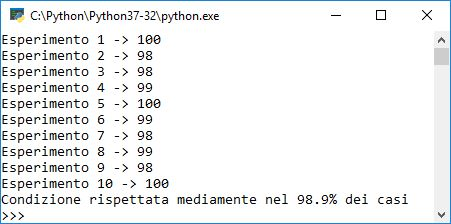
\includegraphics[width=.9\textwidth]{resPython}
				\caption{esecuzione del test di validazione}
				\label{fig:resPython}
			\end{center}
		\end{figure}
	
		Come si vede in \cref{fig:resPython}, in media, in più del $98\%$ delle esecuzioni l'equazione è effettivamente verificata.	Possiamo quindi affermare che la condizione imposta sia assolutamente plausibile. 	 		

	\section{Contromisure ai timing attacks}
	Illustriamo adesso alcune precauzioni che possono essere prese per difendersi dai timing attacks.
	
	\subsection*{Computazione indipendente da input o chiavi}
		La prima contromisura che può essere applicata è quella di rendere indipendente dagli input o dalla chiave il tempo d'esecuzione delle funzioni più critiche. Nel momento in cui una di queste funzioni dovesse aver bisogno di utilizzare tali dati, quella funzione deve essere implementata in modo tale da restituire un tempo di computazione costante (in termini di cicli di clock).
		
		Questa tecnica risolve completamente il problema dei timing attacks, ma diminuisce le prestazioni del programma. Questo è dovuto al fatto che alcune ottimizzazioni proposte nel tempo per velocizzare la computazione di tali funzioni dipendono da una particolare gestione degli input o della chiave, e quindi non possono essere applicate.
		
	\subsection*{Blinding}
		Un'altra contromisura, introdotta da \emph{Chaum} in \cite{chaum1983blind}, consiste nel "nascondere" l'utilizzo di input esterni e di chiavi, modificandoli in maniera opportuna. Ad ogni esecuzione, ad esempio, potrebbe essere aggiunta una quantità casuale alla chiave o all'esponente utilizzato nell'esponenziazione modulare che, modificandoli, renda sempre diverso il tempo di computazione.
		
		Nell'utilizzare questa tecnica è necessario prestare attenzione al fatto che le quantità aggiunte non presentino a loro volta delle regolarità statistiche che potrebbero essere analizzate dall'attaccante, rilevate e compensate.
		
	\subsection*{Rimozione delle istruzioni di branch}
		In \cite{schwabe2016counter}, \emph{Schwabe} propone di implementare funzioni sensibili senza utilizzare istruzioni di branch. Eliminare tali istruzioni permette infatti di uniformare i tempi di esecuzione rendendo molto più difficile l'attuazione dei timing attacks.
		
		Se ad esempio prendiamo il \cref{list:timing} ci accorgiamo che il programma ha tempi di esecuzione diversi in base al valore del segreto.
		
		\begin{center}
			\begin{lstlisting}[language={C},caption={codice da proteggere},label={list:timing}]
				if (secret) {
					r = doA(); /* long operation*/
				} else {
					r = doB(); /*short operation*/
				}
			\end{lstlisting}
		\end{center}
		
		Per osservare i risvolti pratici di questo problema, prendiamo un'implementazione di una delle operazioni più critiche di RSA: l'esponenziazione modulare (\cref{list:square1}).
		
		\begin{center}
			\begin{lstlisting}[language={C},caption={RSA, esponenziazione modulare v1},label={list:square1}]
				typedef unsigned long long uint64;
				typedef uint32_t uint32;
				uint32 modexp(uint32 a, uint32 mod, unsigned char exp[4]) {
					int i,j;
					uint32 r = 1;
					for(i=3;i>=0;i--) {
						for(j=7;j>=0;j--) {
							r = ((uint64)r*r) % mod;
							if(exp[i] & (1<<j))
								r = ((uint64)a*r) % mod;
						}
					}
					return r;
				}
			\end{lstlisting}
		\end{center}
		
		Le istruzioni a riga $9-10$ che eseguono una moltiplicazione ed una riduzione modulare solo se l'i-esimo bit dell'esponente è pari a $1$, sono quelle che potrebbero fornire le informazioni temporali all'attaccante.
		
		La prima modifica che può venire in mente per risolvere questo problema è di far eseguire le stesse operazioni ad entrambi i rami della branch, modificando la funzione come nel \cref{list:square2}. In questo modo, a prescindere dal risultato del controllo, verranno effettuate comunque una moltiplicazione ed una riduzione modulare, uniformando il tempo di esecuzione.
		
		\begin{center}
			\begin{lstlisting}[language={C},caption={RSA, esponenziazione modulare v2},label={list:square2}]
			typedef unsigned long long uint64;
			typedef uint32_t uint32;
			uint32 modexp(uint32 a, uint32 mod, unsigned char exp[4]) {
				int i,j;
				uint32 r = 1, t;
				for(i=3;i>=0;i--) {
					for(j=7;j>=0;j--) {
						r = ((uint64)r*r) % mod;
						if(exp[i] & (1<<j)){
							r = ((uint64)a*r) % mod;
						} else {
							t = ((uint64)a*r) % mod;
						}
					}
				}
				return r;
			}
			\end{lstlisting}
		\end{center}
	
		Questa soluzione è purtroppo inefficace perché qualunque compilatore si accorgerebbe del fatto che la variabile \texttt{t} non viene mai utilizzata, ottimizzando il codice con la rimozione di quell'istruzione. Se anche evitassimo tutte le ottimizzazioni da parte del compilatore (subendo una notevole perdita di prestazioni generali del programma), potremmo comunque non ottenere un tempo costante a causa di altre ottimizzazioni (inevitabili) a livello di processore, come ad esempio la \emph{branch prediction}.
		
		La soluzione proposta è quella di eliminare completamente l'istruzione di branch come nel \cref{list:square3}.
		
		\begin{center}
			\begin{lstlisting}[language={C},caption={RSA, esponenziazione modulare v3},label={list:square3}]
			uint32 modexp(uint32 a, uint32 mod, const unsigned char exp[4]) {
				int i,j;
				uint32 r = 1,t;
				for(i=3;i>=0;i--) {
					for(j=7;j>=0;j--) {
						r = ((uint64)r*r) % mod;
						t = ((uint64)a*r) % mod;
						cmov(&r, &t, (exp[i] >> j) & 1);
					}
				}
				return r;
			}
			\end{lstlisting}
		\end{center}
	
		In questa implementazione vengono sempre eseguite entrambe le operazioni (sia su \texttt{r} che su \texttt{t}) e si nota l'utilizzo dell'istruzione assembly \texttt{cmov} (\emph{conditional move}). Questa istruzione non fa uso di alcuna predizione sulla branch ed ha bisogno sia del valore di \texttt{r} che del valore \texttt{t}, che quindi non possono essere ottimizzati.
		
%\chapter{Cache attacks}
	\index{Cache attacks}I timing attacks sono molto utilizzati per effettuare attacchi sulla cache del processore. Approfondiremo questo argomento, ma prima è necessario presentare e chiarire alcune nozioni fondamentali su questo componente. 
	
	\section{La cache del processore}
		Solitamente ogni programma tende a riutilizzare nel tempo un dato contenuto allo stesso indirizzo di memoria (\emph{località temporale}\index{Località temporale}) e più dati localizzati in indirizzi vicini nella memoria (\emph{località spaziale}\index{Località spaziale}). Ad esempio, se nel programma è presente un loop, lo stesso codice sarà eseguito più e più volte nel tempo, verosimilmente con gli stessi dati.
		
		Dato che la differenza di velocità tra le memorie e la capacità di calcolo dei processori aumenta sempre di più \cite{hennessy2011computer}, la banda del bus di comunicazione e la velocità di accesso alla memoria principale sono diventati un fattore limitante sul throughput generale del processore. Per sfruttare al meglio la località temporale e superare questo collo di bottiglia viene utilizzate la cache\index{Cache}. 
		
		Essa è infatti un piccolo banco di memoria molto veloce (e molto costoso) sito all'interno di ogni core che il processore utilizza per immagazzinare i valori delle celle di memoria lette più recentemente. 
		
		\subsection{Struttura della cache}
			I processori moderni hanno generalmente due livelli di cache per ogni core chiamati rispettivamente L$1$ e L$2$ ed un terzo livello chiamato \ac{LLC} o L$3$ condiviso tra i tutti i core (nella \cref{tab:processori} sono riportate le dimensioni delle varie memorie di alcuni processori). 
			
			\begin{table}[]
				\footnotesize
				\centering
				\begin{tabular}{|c|c|c|c|c|c|c|} \hline
					Casa		& Nome				& Core	& L$1$						& L$2$						& L$3$					& Prezzo (\$)	\\ \hline \hline
					Intel		& i$3$-$530$		& $2$	& $2$ x $64$ \kilobyte		& $2$ x $512$\kilobyte		& $1$ x $4$ \megabyte	& $113$			\\ \hline
								& i$5$-$6685$R		& $4$	& $4$ x $64$ \kilobyte		& $4$ x $256$\kilobyte		& $1$ x $6$ \megabyte	& $288$			\\ \hline
								& i$7$-$6950$X		& $10$	& $10$ x $64$ \kilobyte		& $10$ x $256$\kilobyte		& $1$ x $25$ \megabyte	& $1723$		\\ \hline
								& i$9$-$8950$HK		& $6$	& $6$ x $64$ \kilobyte		& $6$ x $256$\kilobyte		& $1$ x $12$ \megabyte	& $583$			\\ \hline
					AMD			& A$4$ Pro-$3350$B	& $4$	& $4$ x $64$ \kilobyte		& $1$ x $2$\megabyte		& -						& -				\\ \hline
								& Athlon $5370$		& $4$	& $4$ x $64$ \kilobyte		& $1$ x $2$\megabyte		& -						& $55$			\\ \hline
								& Epyc $7251$		& $8$	& $8$ x $96$ \kilobyte		& $8$ x $512$\kilobyte		& $32$ \megabyte		& $475$			\\ \hline
				\end{tabular}
				\caption{caratteristiche di alcuni processori}
				\label{tab:processori}
			\end{table}
			
			Considerando che l'accesso alla memoria principale in media impiega dai $50$ ai $150$\emph{ns}, mentre l'accesso alla cache L$1$ utilizza un tempo nell'ordine degli $0.3$\emph{ns}, si può capire l'enorme differenza di prestazioni che possono essere raggiunte utilizzando questo tipo di memoria. 
			
			Da questo momento in poi parleremo di \emph{cache hit} quando il dato richiesto è presente in cache e viene letto molto velocemente e di \emph{cache miss} quando invece dovrà essere recuperato dalla memoria principale.
		
			Nella \cref{fig:cachei5} si può vedere l'architettura del processore quadcore Intel Core i$5$-$3470$. La gerarchia delle cache è organizzata in una memoria L$1$ di $64$\kilobyte \ (divisa in $32$\kilobyte \ per le istruzioni e $32$\kilobyte \ per i dati), una memoria L$2$ da $256$\kilobyte \ ed una memoria L$3$ da $6$\megabyte.
			
			Andiamo ad analizzare più nel dettaglio le caratteristiche di una singola cache\cite{ge2016survey,yarom2014flush+}.
			
			\begin{figure}[h]
				\begin{center}
					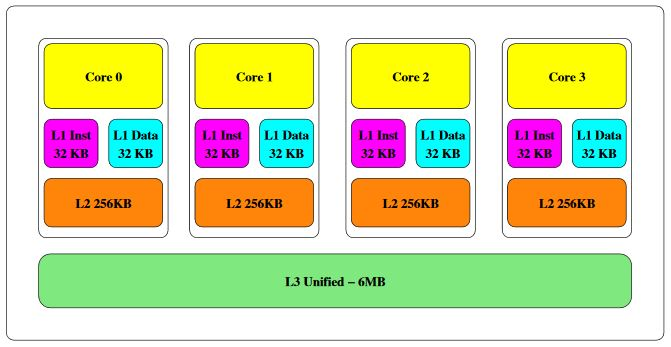
\includegraphics[scale=0.6]{cachei5}
					\caption{architettura del processore Intel Core i$5$-$3470$}
					\label{fig:cachei5}
				\end{center}
			\end{figure}
			
			\subsubsection{Cache lines}
				\index{Cache lines}Per sfruttare anche la località spaziale le caches sono divise in lines. Una cache line contiene un blocco di byte adiacenti (generalmente di dimensione congrua ad una potenza di due) caricati dalla memoria. Se uno qualunque dei byte deve essere rimosso (si parla di \emph{evicting}\index{Evict}) per far spazio ad un altro dato, viene rimossa l'intera line.
				
			\subsubsection{Associatività}
				Teoricamente una qualunque posizione di memoria può essere mappata in una qualunque cache line ed una cache ad \emph{n} lines potrebbe contenere \emph{n} linee qualunque della memoria. Questo tipo di cache viene chiamato \emph{fully-associative cache}\index{Fully-associative cache} ed è la migliore in teoria perché può sempre essere usata al massimo delle sue capacità ed i cache miss si hanno solamente quando non c'è più spazio libero nella cache. Tuttavia, nella pratica, tutto ciò si traduce in un controllo in parallelo di tutte le linee che aumenta la complessità architetturale e il consumo di energia.
				
				L'estremo opposto è chiamato \emph{direct-mapped cache}\index{Direct-mapped cache}. In questo sistema ogni locazione di memoria può stare in una sola cache line, ben determinata da una funzione di indicizzazione. Due locazioni di memoria che mappano sulla stessa cache line non possono essere immagazzinate contemporaneamente e il loading di una comporta inevitabilmente l'evicting dell'altra. Questo potrebbe portare ad avere dei miss anche con la cache semivuota.
				
				\begin{figure}
					\begin{center}
						
\includegraphics[scale=.5]{cache}
						\caption[$8$-way associative cache]{un esempio di $8$-way associative cache con otto set formati ognuno da $4$ line. La dimensione totale sarà $S*B*W \ byte$}
						\label{fig:cache}
					\end{center}
				\end{figure}
				
				Concretamente viene utilizzata una via di mezzo tra queste due soluzioni chiamata \emph{set-associative cache}\index{Set-associative cache}. La cache viene divisa in \emph{sets} (generalmente di dimensione compresa tra due e ventiquattro lines) in cui ogni indirizzo viene controllato in parallelo come in una fully-associative cache. Per determinare in quale set viene mappato un blocco di memoria viene usata una funzione del suo indirizzo, come per una direct-mapped cache. Una cache con \emph{S} line sets viene chiamata \emph{S-way associative} (\cref{fig:cache}). 
				
				In \cref{fig:cachefill} possiamo vedere un esempio di direct-mapped e $2$-way associative cache. 
				
				Nella prima, la funzione di indicizzazione potrebbe essere: $$\text{cache memory index} = \text{main memory index}\ \% \ 4$$ Supponiamo adesso che in cache sia presente il dato \emph{x} contenuto all'indirizzo $0$ della memoria principale. La richiesta del dato \emph{y} contenuto all'indirizzo $4$ provocherà l'evict di \emph{x}.
				
				Nella seconda, la funzione di indicizzazione potrebbe essere: $$\text{cache memory index} = \text{main memory index}\ \% \ 2$$ In questo caso però, dal momento che per ogni set è possibile salvare due line contemporaneamente, la richiesta del dato \emph{y} non provocherebbe l'evict del dato \emph{x} già presente in cache, ma sarebbero entrambi presenti nel set $0$: l'uno con indice $0$ e l'altro con indice $1$.
				
				Si può notare che le direct-mapped e le fully-associative cache non sono altro che casi particolari di set-associative cache, rispettivamente $1$-way associative ed N-way associative (dove N è il numero totale di lines della cache).
				
				\begin{figure}
					\begin{center}
						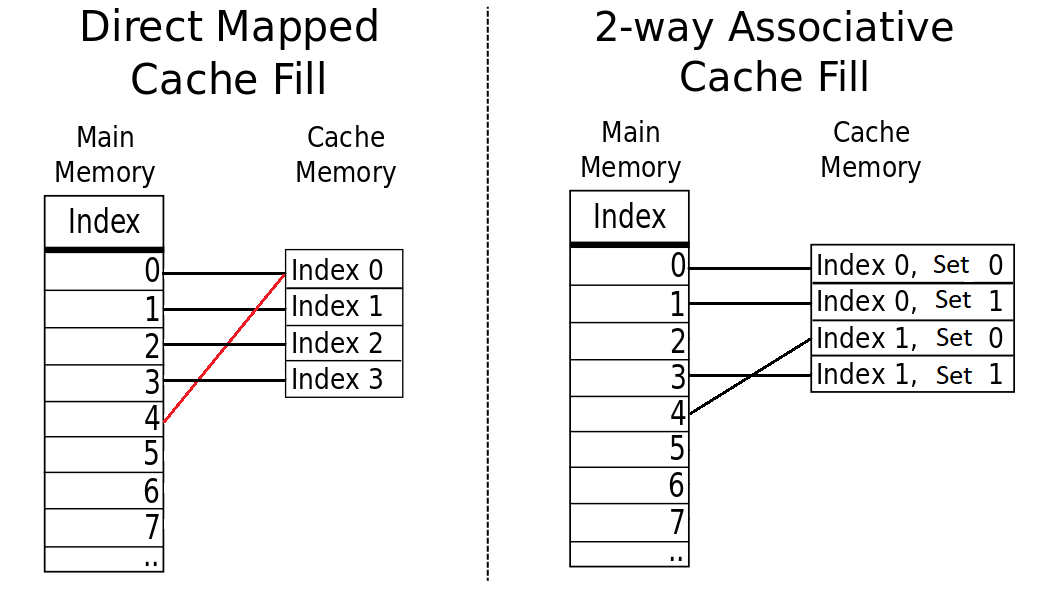
\includegraphics[scale=.35]{cachefill}
						\caption{schemi di associatività della cache}
						\label{fig:cachefill}
					\end{center}
				\end{figure}
				
			\subsubsection{Inclusività}
				Una caratteristica che verrà sfruttata per montare l'attacco è l'\emph{inclusività}\index{Inclusività}. 
				
				Ogni livello superiore di cache contiene un sottoinsieme dei dati contenuti nel livello direttamente inferiore. Per mantenere questa caratteristica, quando viene eseguito un evicting di un dato da un livello inferiore, questo viene rimosso anche da tutti i livelli superiori.
				
				Se ad esempio effettuiamo un evicting di una line contenuta nella cache L$3$, lo stesso dato, se presente, verrà rimosso anche dalla L$1$ e dalla L$2$.
				
	\section{Cache attacks}
		Per capire come funzionano la maggior parte degli attacchi alle cache prendiamo in considerazione un array di dati. Quando un elemento di questo array viene letto, o si verifica una hit o una miss.
		
		La differenza tra le due esecuzioni è notevole (diversi ordini di grandezza) ed è questa l'informazione utilizzata nell'attacco.
		
		\subsection{Tassonomia}
			Una prima classificazione dei cache attacks si basa sullo stato della cache al momento dell'attacco \cite{canteaut2006understanding}.
			
			\begin{itemize}
				\item \emph{Empty initial state}\index{Empty initial state} (reset attacks): questi attacchi si basano sull'assunzione che nessun dato che dovrà essere utilizzato dalla vittima è presente in cache.
				\item \emph{Forged initial state}\index{Forged initial state} (initialization attacks): in questo caso l'attaccante deve essere in grado di portare la cache in uno stato noto prima di poter effettuare l'attacco.
				\item \emph{Loaded initial state}\index{Loaded initial state} (micro-architecture attacks): la cache contiene tutti i dati necessari alla vittima per eseguire il programma.
			\end{itemize}
		
			Nello stesso lavoro si fornisce una classificazione anche in base al tipo di cache miss:
			
			\begin{itemize}
				\item \emph{Cold start misses}\index{Cold start misses}: questo tipo di miss si ottiene quando il dato viene letto per la prima volta e quindi non è ancora mai stato caricato in cache.
				\item \emph{Capacity misses}\index{Capacity misses}: questo tipo di miss si ottiene quando si cerca di accedere a porzioni di memoria più grandi della dimensione della cache, e che quindi non potranno essere presenti nella cache contemporaneamente.
				\item \emph{Conflict misses}\index{Conflict misses}: questo tipo di miss si ottiene quando un accesso precedente alla nostra richiesta ha provocato la eviction del dato di interesse (che era presente in cache).
			\end{itemize}
			
			In \cite{lipp2016armageddon,ge2016survey} si classificano gli attacchi in base all'approccio utilizzato:
			
			\begin{figure}
				\begin{center}
					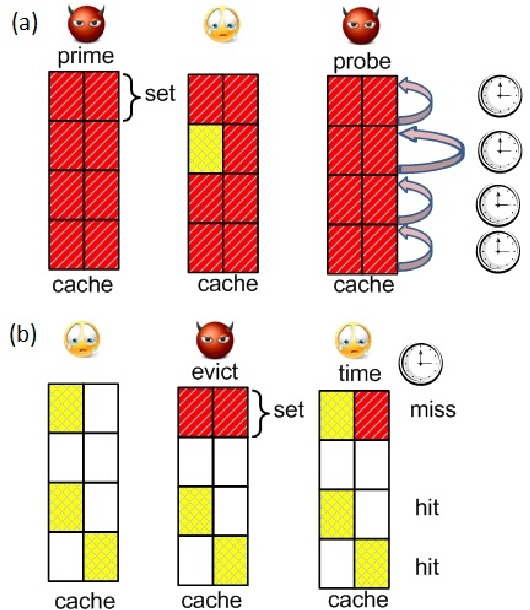
\includegraphics[scale=0.4]{cacheattacks}
					\caption{schema di attacco Prime+Probe (a) e Evict+Time(b)}
					\label{fig:cacheattacks}
				\end{center}
			\end{figure}
			
			\begin{itemize}
				\item \emph{Prime+Probe}\cite{osvik2006cache}\index{Prime+Probe}: questo è un attacco di tipo forged initial state. L'attaccante precarica uno o più set della cache con dati propri e, dopo l'esecuzione della funzione vittima, prova a riaccedere ai dati precaricati. Se la funzione vittima non ha utilizzato lines mappate nei cache set occupati dall'attaccante, egli otterrà solo cache hit. Al contrario, se c'è stato l'evict di qualche line, allora capirà quale line ha utilizzato la vittima. Lo schema di questo attacco e del seguente è visibile in \cref{fig:cacheattacks}.
				\item \emph{Evict+Time}\cite{osvik2006cache}\index{Evict+Time}: questo attacco è di tipo loaded initial state e suppone che tutti i dati che servono alla vittima siano già in cache. Questa condizione può essere ottenuta facendo eseguire una prima volta la funzione vittima. Dato questo presupposto, l'attaccante fa eseguire la funzione alla vittima calcolandone il tempo di esecuzione. Successivamente esegue un evict di un cache set caricando dati propri e fa eseguire nuovamente la funzione vittima. Se il tempo di questa ultima esecuzione è maggiore del precedente vuol dire che la funzione ha cercato di utilizzare un dato che è stato rimosso dalla cache ed ha dovuto aspettare di recuperarlo dalla memoria principale.
				\item \emph{Flush+Reload}\cite{yarom2014flush+}\index{Flush+Reload}: questo attacco è una variante di Prime+Probe. L'attacco si divide in tre fasi: Nella prima fase l'attaccante esegue l'evict della line a cui è interessato utilizzando l'istruzione \emph{clflush}\cite{intel64and}\index{Clflush} che invalida il dato su tutti i livelli della cache; nella seconda fase aspetta che la vittima esegua la propria funzione; nella terza fase l'attaccante ricarica la line che aveva rimosso. Se la risposta è veloce vuol dire che la vittima ha portata nella cache la line interessata durante l'esecuzione della sua funzione.
				\item \emph{Evict+Reload}\cite{gruss2015cache}\index{Evict+Reload}: una variante del Flush+Reload che utilizza la eviction al posto dell'istruzione di flush. Questa variante è poco utile se il processore sotto attacco è della famiglia x$86$ in quanto l'istruzione \emph{clflush} non richiede alcun privilegio, mentre assume un certo rilievo se l'obiettivo è quello di attaccare un processore che non fornisce, nel suo set di istruzioni, una istruzione non privilegiata in grado di rimuovere dati dalla cache (come ad esempio quelli della famiglia ARM).
				\item \emph{Flush+Flush}\cite{gruss2016flush+}\index{Flush+Flush}: diversamente da tutti i precedenti approcci, in questo caso non si esegue nessun accesso alla memoria. L'attaccante si basa solamente sul tempo impiegato dall'istruzione \emph{clflush}. In \cite{lipp2016armageddon} si fa vedere come l'esecuzione di questa funzione abbia tempi differenti se chiamata su un indirizzo presente o meno in cache.  
			\end{itemize}
		
		\section{L'attacco ad AES}
			Un ottimo esempio di come sono stati messi in pratica buona parte dei concetti visti fino ad ora è l'attacco ad \ac{AES} portato da \emph{Osvik, Shamir \text{e} Tromer} in \cite{osvik2006cache}.
			
			\subsection{AES}
				\ac{AES}\index{AES} è un algoritmo di cifratura a blocchi, a chiave simmetrica, scelto come standard dagli Stati Uniti d'America dalla \ac{FIPS} nel documento PUB $197$\cite{pub2001197}. Viene considerato a tutti gli effetti il successore di \ac{DES}, in via di abbandono a causa della sua ormai provata insicurezza\cite{kumar2006breaking,gilmore1998cracking}. La seguente spiegazione dell'algoritmo è presa da \cite{stallings2012computer}.
				
				\ac{AES} utilizza blocchi di $128$ bit e una chiave che può essere lunga $128$, $192$ o $256$ bit ($128$ è la lunghezza più comunemente implementata).
			
				L'input dell'algoritmo è un singolo blocco di $128$ bit che nello standard viene trattato come una matrice quadrata di byte (come la chiave a $128$ bit). Questo blocco viene copiato in un array chiamato \emph{stato} che verrà modificato ad ogni round di encryption/decryption. Alla fine dell'ultimo round, lo stato finale sarà copiato in una matrice che rappresenterà il risultato della computazione. La chiave viene espansa in un array di word (della lunghezza di quattro byte) ricavando $44$ word dai $128$ bit di partenza. Ad ogni round verranno prese di volta in volta quattro word ($128$ bit) e verranno utilizzate come chiave per quel round.
				
				Senza scendere troppo nell'implementazione è importante capire le quattro operazioni effettuate ad ogni round (\cref{fig:operations}):
				
				\begin{itemize}
					\item \emph{Substitute byte}: tramite una tabella (\emph{S-Box}) vengono sostituiti, byte per byte, tutti i byte del blocco.
					\item \emph{Shift row}: viene effettuata una permutazione delle righe della matrice
					\item \emph{Mix columns}: vengono modificate le colonne moltiplicandole per un polinomio fisso $c(x)$.
					\item \emph{Add round key}: viene effettuato uno XOR tra il blocco corrente e la chiave di round.
				\end{itemize}
			
				\begin{figure}
					\begin{center}
						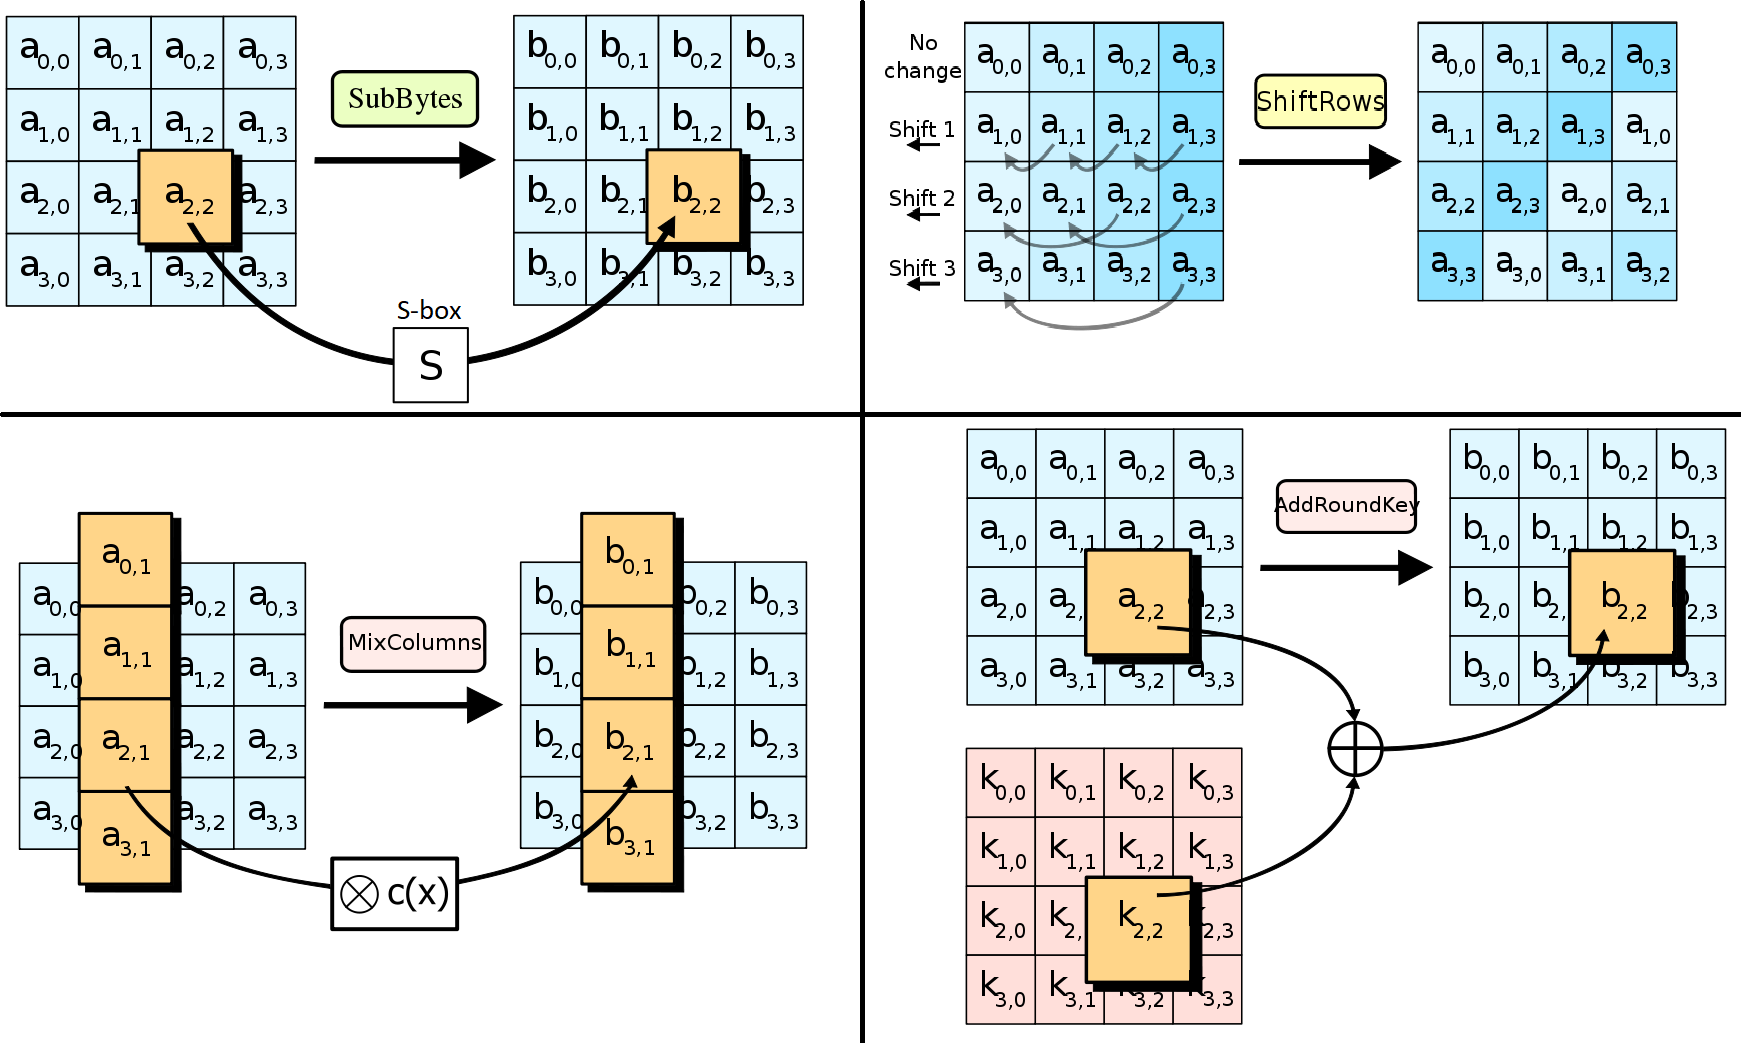
\includegraphics[width=\textwidth]{aesOperations}
						\caption{schema delle operazioni effettuate da AES}
						\label{fig:operations}
					\end{center}
				\end{figure}
			
				Come si vede in \cref{fig:aes} l'algoritmo inizia con un \emph{add round key} seguito da nove round in cui vengono effettuate tutte e quattro le operazioni. L'ultimo round (il decimo) è composto solo da tre operazioni (non viene effettuata la \emph{mix columns}). 
				
				\begin{figure}
					\begin{center}
						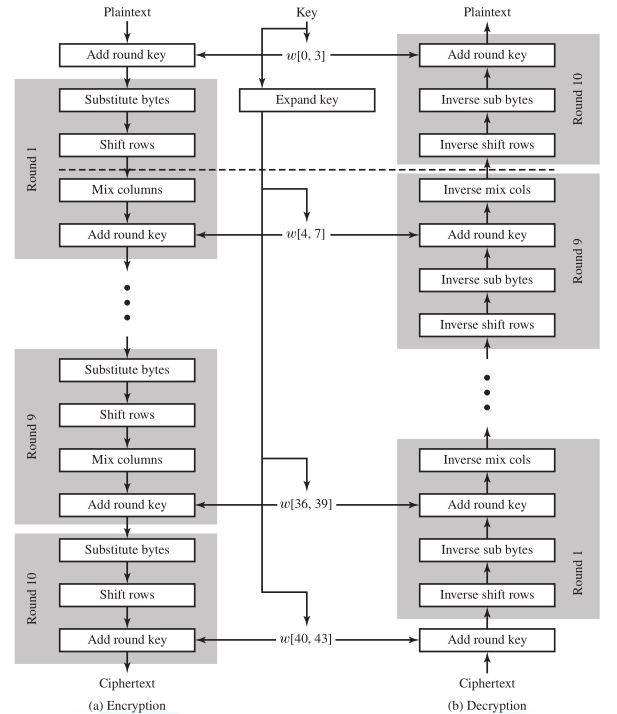
\includegraphics[width=.9\textwidth]{AES}
						\caption{schema di funzionamento di AES}
						\label{fig:aes}
					\end{center}
				\end{figure}
				
			\subsection{Implementazione e uso della memoria}
				Quello descritto finora è il funzionamento teorico di \ac{AES}. Tutto l'algoritmo sarebbe eseguibile tramite semplici operazioni algebriche, ma in realtà vengono create (dal programmatore o durante l'inizializzazione del sistema) otto tabelle di lookup per ottimizzare le performance. Chiameremo tali tabelle $\mathcal{T}_0, \mathcal{T}_1, \mathcal{T}_2, \mathcal{T}_3$ e $\mathcal{T}_{0}^{(10)}, \mathcal{T}_{1}^{(10)}, \mathcal{T}_{2}^{(10)}, \mathcal{T}_{3}^{(10)}$. Ognuna di queste tabelle contiene $256$ word da quattro byte. La chiave (sedici byte) $\mathbf{k} = (k_1,\dots ,k_{16})$ viene estesa per formare dieci chiavi (una per ogni round) $\mathbf{K}^{(r)}$ per $r = 1,\dots ,10$. Le chiavi vengono suddivise in quattro word di quattro byte ciascuna $\mathbf{K}^{(r)}=\left( K_{0}^{(r)},K_{1}^{(r)},K_{2}^{(r)},K_{3}^{(r)}\right) $. Dato un plaintext di sedici byte $\mathbf{p}=(p_0, \dots , p_{15})$ la funzione di encryption calcola uno stato intermedio $\mathbf{x}^{(r)}=(x_{0}^{(r)}, \dots , x_{15}^{(r)})$ ad ogni round r. Lo stato iniziale $\mathbf{x}^{(0)}$ viene calcolato come $x_{i}^{(0)} = p_i \oplus k_i \text{ con }(i = 0,\dots ,15)$. I successivi nove round vengono calcolati aggiornando lo stato intermedio secondo le seguenti equazioni: $$\forall r \in (0,\dots,8):$$
				{
					\scriptsize
					\begin{center}
						\begin{tabular}{ccc}
							$\left(x_{0}^{(r+1)},x_{1}^{(r+1)},x_{2}^{(r+1)},x_{3}^{(r+1)}\right)$ & $\leftarrow$ & $\mathcal{T}_{0}\left[x_{0}^{(r)}\right] \oplus \mathcal{T}_{1}\left[x_{5}^{(r)}\right] \oplus \mathcal{T}_{2}\left[x_{10}^{(r)}\right] \oplus \mathcal{T}_{3}\left[x_{15}^{(r)}\right]\oplus K_{0}^{(r+1)}$\\
							$\left(x_{4}^{(r+1)},x_{5}^{(r+1)},x_{6}^{(r+1)},x_{7}^{(r+1)}\right)$ & $\leftarrow$ & $\mathcal{T}_{0}\left[x_{4}^{(r)}\right] \oplus \mathcal{T}_{1}\left[x_{9}^{(r)}\right] \oplus \mathcal{T}_{2}\left[x_{14}^{(r)}\right] \oplus \mathcal{T}_{3}\left[x_{3}^{(r)}\right]\oplus K_{1}^{(r+1)}$\\
							$\left(x_{8}^{(r+1)},x_{9}^{(r+1)},x_{10}^{(r+1)},x_{11}^{(r+1)}\right)$ & $\leftarrow$ & $\mathcal{T}_{0}\left[x_{8}^{(r)}\right] \oplus \mathcal{T}_{1}\left[x_{13}^{(r)}\right] \oplus \mathcal{T}_{2}\left[x_{2}^{(r)}\right] \oplus \mathcal{T}_{3}\left[x_{7}^{(r)}\right]\oplus K_{2}^{(r+1)}$\\
							$\left(x_{12}^{(r+1)},x_{13}^{(r+1)},x_{14}^{(r+1)},x_{15}^{(r+1)}\right)$ & $\leftarrow$ & $\mathcal{T}_{0}\left[x_{12}^{(r)}\right] \oplus \mathcal{T}_{1}\left[x_{1}^{(r)}\right] \oplus \mathcal{T}_{2}\left[x_{6}^{(r)}\right] \oplus \mathcal{T}_{3}\left[x_{11}^{(r)}\right]\oplus K_{3}^{(r+1)}$
						\end{tabular}
					\end{center}
				}
			
				L'ultimo round viene calcolato con $r = 9$ ma, al posto di usare $\mathcal{T}_0, \mathcal{T}_1, \mathcal{T}_2, \mathcal{T}_3$ verranno usate $\mathcal{T}_{0}^{(10)}, \mathcal{T}_{1}^{(10)}, \mathcal{T}_{2}^{(10)}, \mathcal{T}_{3}^{(10)}$. Il risultante $\mathbf{x}^{10}$ sarà il ciphertext.
				
				Paragonando questa implementazione con la formulazione algebrica teorica di \ac{AES} si può vedere che le otto tabelle di lookup vengono usate per effettuare le quattro operazioni di ogni round in maniera immediata. L'ultimo round ha bisogno di quattro tabelle diverse perché non viene eseguita l'operazione \emph{mix columns}.
				
				L'attacco (i cui dettagli possono essere trovati nell'articolo) si basa proprio sul cercare di capire i valori $x_{i}^{(r)}$ usati come indici nelle varie tabelle che di volta in volta verranno caricate in cache. Tali valori vengono recuperati tramite attacchi evict+time o prime+probe.
		
		\section{Contromisure possibili}
			Le difese da questo tipo di attacchi sono sia software che hardware e si dividono in cinque grandi famiglie \cite{ge2016survey}:
			
			\begin{description}
				\item[Tecniche a tempo costante:] l'idea di base è quella di rendere il comportamento del codice che esegue operazioni critiche indipendente dai dati. Per esempio cercando di rendere una funzione crittografica indipendente sia dalla chiave che dall'input. Questo può essere ottenuto facendo eseguire istruzioni inutili per uniformare il tempo di esecuzione o accedendo casualmente alla memoria per confondere l'attaccante sull'utilizzo della cache. 
				
				Queste soluzioni ovviamente portano ad una drastica perdita di prestazioni. Il tempo di esecuzione dovrà infatti tendere al tempo di esecuzione massimo ogni volta che sarà necessario richiamare la funzione.
				
				L'altro grande problema di questo tipo di soluzioni è quello della differenza di risultati su hardware differenti. Ad esempio \emph{Cock et al.}\cite{cock2014last} hanno dimostrato che la correzione a tempo costante adottata per mitigare l'attacco \emph{Lucky} $13$\cite{al2013lucky} in OpenSSL $1.0.1e$ non risolve il problema se fatto girare su un processore ARM AM$3358$. 
				\item[Inserimento di rumore:] questa famiglia di contromisure tende a rendere inutilizzabili le misurazioni ottenute dall'attaccante inserendo in ogni evento osservabile da qualsiasi processo una quantità di rumore tale da renderne impossibile una qualunque analisi\cite{hu1992reducing}. Questa soluzione, in teoria, riesce a risolvere completamente il problema, ma è stato dimostrato\cite{cock2014last} che in pratica non è applicabile. La quantità di rumore da produrre e da aggiungere alla computazione è talmente elevata che il sistema impiegherebbe la maggior parte delle sue risorse in questa operazione piuttosto che nella effettiva computazione del programma.
				\item[Imporre determinismo:] in questo caso si cerca di eliminare qualsiasi tipo di misura sul tempo eliminando completamente le variazioni di tempo visibile. Ad esempio in \cite{aviram2012efficient} si propone di eliminare completamente l'accesso al tempo reale fornendo all'esterno solamente un clock virtuale il cui avanzamento è completamente deterministico e indipendente dalle azioni di componenti vulnerabili. Per ottenere questo risultato si cerca di sincronizzare tutti i clock con l'esecuzione di un singolo processo, indipendente da input o azioni esterne, che esegue in tempo costante.
				\item[Suddividere il tempo:] una delle soluzioni maggiormente utilizzate è quella in cui si cerca di suddividere il tempo in sezioni nelle quali si fornisce un accesso esclusivo all'hardware condiviso. Ci sono diverse tecniche per ottenere questo risultato, una ad esempio è lo svuotamento completo della cache ad ogni context switch (\emph{cache flushing}\index{Cache flushing}\cite{zhang2013duppel}). Questo ovviamente porta ad una perdita in prestazioni molto grande, pertanto si è pensato di eseguire il flushing della cache non ad ogni context switch, bensì solo al passaggio da processi sensibili a processi inaffidabili (\emph{lattice scheduling}\index{Lattice scheduling}\cite{denning1976lattice}). Un'altra soluzione \cite{varadarajan2014scheduler} sfrutta la necessità dell'attaccante di analizzare frequentemente lo stato della cache della vittima: tale necessità (tipica degli attacchi di tipo Prime+Probe ad esempio) può essere negata imponendo un tempo minimo di esecuzione per le componenti vulnerabili, rendendo quindi impossibile la loro prelazione entro dato tempo.
				\item[Suddividere le risorse hardware:] attacchi eseguiti da processi concorrenti possono essere evitati solamente suddividendo adeguatamente le risorse hardware tra i vari processi. Per quanto riguarda la cache sono state avanzate varie proposte. Percival\cite{percival2005cache} suggerisce di suddividere la cache L$1$ tra i vari processi in modo tale da non permettere ad un processo di accedere o rimuovere lines utilizzate da un altro. Wang e Lee\cite{wang2007new} propongono invece la \emph{partition-locked cache}, un meccanismo hardware che permette di assegnare dei lock ad alcune lines contenenti dati particolarmente sensibili in maniera tale da non poter essere rimosse (ad esempio le tabelle di lookup di \ac{AES}).				 
			\end{description}
%\chapter{SPECTRE attacks}

	\begin{wrapfigure}{l}{0.4\textwidth}
		
\includegraphics[width=0.38\textwidth]{spectre}
		\caption{il logo di SPECTRE}
		\label{fig:spectre}
	\end{wrapfigure}

	\index{Spectre}In questo capitolo verrà presentato il progetto \emph{SPECTRE}\cite{kocher2018spectre} (il cui logo è rappresentato in \cref{fig:spectre}): una famiglia di attacchi molto recenti che sfruttano una vulnerabilità presente nella maggior parte dei processori moderni (Intel, AMD e ARM) e per i quali, al momento attuale, non esistono contromisure tranne l'utilizzo di alcuni accorgimenti in fase di programmazione (come vedremo più avanti).
	
	Si parla di famiglia di attacchi perché di questo attacco esistono cinque varianti, tutti documentati con il proprio codice \ac{CVE} nello \emph{Standard for Information Security Vulnerability Names} gestito dalla \href{https://www.mitre.org/}{MITRE Corporation}. Le varianti sono le seguenti:
	
	\begin{itemize}
		\item [v1:] bounds check bypass \href{https://cve.mitre.org/cgi-bin/cvename.cgi?name=CVE-2017-5753}{(CVE-2017-5753)}
		\item [v2:] branch target injection \href{https://cve.mitre.org/cgi-bin/cvename.cgi?name=CVE-2017-5715}{(CVE-2017-5715)}
		\item [v3:] using speculative reads of inaccessible data \href{https://cve.mitre.org/cgi-bin/cvename.cgi?name=CVE-2017-5754}{(CVE-2017-5754)}
		\item [v3a:] using speculative reads of inaccessible data, aka "rogue system register read" \href{https://cve.mitre.org/cgi-bin/cvename.cgi?name=CVE-2018-3640}{(CVE-2018-3640)}
		\item [v4:] speculative bypassing of stores by younger loads despite the presence of a dependency \href{https://cve.mitre.org/cgi-bin/cvename.cgi?name=CVE-2018-3639}{(CVE-2018-3639)}
	\end{itemize}
	
	Nel resto di questo lavoro ci focalizzeremo sulla prima variante di questa tipologia di attacchi.
	
	La principale caratteristica che viene sfruttata in questa variante è la cosiddetta \emph{esecuzione speculativa}, una funzione presente in quasi tutti i processori moderni.
	
	\section{Esecuzione speculativa}
		\index{Esecuzione speculativa}L'esecuzione speculativa è una tecnica utilizzata dai processori per ottenere un miglioramento delle prestazioni. Essa consiste nel cercare di "predire" il risultato di una branch basandosi sui risultati ottenuti in precedenza, per poter eseguire anticipatamente alcune istruzioni.
		
		Immaginiamo di essere in campo durante la finale del mondiale di calcio. Stiamo battendo il rigore decisivo. Abbiamo studiato bene il portiere avversario nell'ultimo anno e sappiamo che le dieci volte in cui gli si è presentato davanti un tiratore mancino (come lo siamo noi) si è sempre tuffato alla sua sinistra ed ha sempre parato il rigore. Avendo fiducia nel nostro studio decidiamo di calciare alla sua destra in maniera non troppo angolata, per non rischiare di sbagliare, certi comunque di spiazzarlo. Sfortunatamente però, questa volta il portiere decide di cambiare lato e para facilmente il nostro rigore facendoci perdere il mondiale.
		
		Quale è stata la cosa che ci ha fatto sbagliare? L'aver speculato sul comportamento del portiere ed aver pensato che il fatto che si fosse sempre tuffato a sinistra nelle occasioni precedenti ed avesse sempre parato il rigore, lo avrebbe portato a farlo di nuovo. Vediamo come riportare questo esempio nel nostro ambito. 
		
		Supponiamo ad esempio che l'esecuzione di un programma dipenda da un controllo su di un valore non presente in cache che quindi deve essere recuperato dalla memoria principale. Questo può portare ad un attesa di svariate centinaia di cicli di clock. Invece di aspettare tutto questo tempo inutilmente, il processore cerca di indovinare il risultato del controllo, salva lo stato attuale dei suoi registri, e procede ad eseguire speculativamente il ramo della branch che ritiene più plausibile (supponiamo il ramo then). Quando poi arriverà il valore effettivo dalla memoria, verrà eseguito il controllo. Se il risultato è quello aspettato (true nel nostro caso), si prosegue con la computazione e saranno stati risparmiati tutti quei cicli di clock che sarebbero stati persi nell'attesa. Se la scelta si rivela sbagliata (false), il processore scarta tutti i risultati dell'esecuzione speculativa, si riporta allo stato che aveva salvato prima del branch ed esegue l'altro ramo (else).
		
		Questa ottimizzazione sembra perfetta in quanto, in caso di successo, si risparmiano molti cicli di clock, mentre in caso di insuccesso il risultato è paragonabile a quello che avremmo ottenuto aspettando il dato senza eseguire alcuna istruzione. Purtroppo vedremo che non è così.
		
		Il responsabile di questa scelta è una piccola unità all'interno del processore chiamata \ac{BP}.
		
		\subsection{Branch predictor}
			\index{Branch Predictor}Esistono svariati tipi di branch predictor; analizziamo il funzionamento di uno dei più semplici: il \emph{one-level branch predictor}\index{One-level branch predictor} a due bit.
			
			\begin{figure}
				\begin{center}
					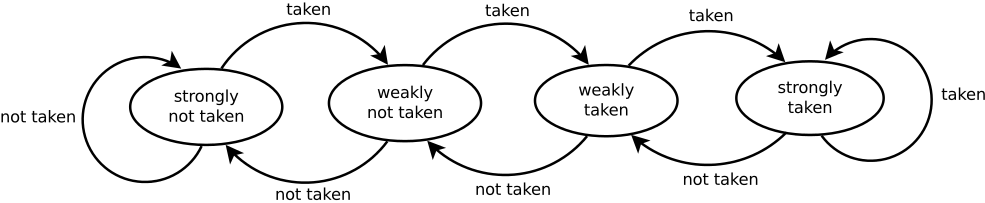
\includegraphics[scale=.35]{bp2bit}
					\caption{automa di decisione di un one-level branch predictor a due bit}
					\label{fig:bp2bits}
				\end{center}
			\end{figure}
		
			Come da schema in \cref{fig:bp2bits} un one-level branch predictor può essere descritto con un semplice automa a quattro stati:
			
			\begin{enumerate}
				\item \emph{Strongly not taken:} in questo stato il \ac{BP} sceglierà il ramo else del branch. In caso di conferma negativa del controllo resterà in questo stato, altrimenti passerà allo stato due.
				\item \emph{Weakly not taken:} in questo stato il \ac{BP} ha già osservato una esecuzione then, ma la sua scelta resterà ancora il ramo else. Se il controllo si rivelerà false, il \ac{BP} tornerà allo stato uno, ma se si rivelerà true andrà allo stato tre dal quale inizierà a scegliere il ramo then.
				\item \emph{Weakly taken:} come detto in precedenza, in questo stato il \ac{BP} inizierà a scegliere il ramo then. Se da questo stato si ottiene un false, torneremo allo stato due, altrimenti passeremo al quattro.
				\item \emph{Strongly taken:} questo stato è il duale dello stato uno. In questa situazione il \ac{BP} sceglierà il ramo then rimanendo in questo stato se otterrà un true, e tornando allo stato tre se otterrà un false (continuando comunque ad eseguire il ramo then).
			\end{enumerate}
		
			In questo caso vediamo come l'esecuzione consecutiva di al più due rami then ci porta sicuramente in uno stato in cui la prossima scelta del \ac{BP} sarà sicuramente il ramo then. Questa informazione sarà molto utile quando dovremo effettuare un training sul \ac{BP} per convincerlo a prendere una certa decisione quando si troverà davanti ad una certa branch.
			
	\section{L'attacco}
		L'attacco SPECTRE induce la vittima ad eseguire speculativamente operazioni che non dovrebbero essere eseguite durante l'esecuzione corretta del programma. Da tali operazioni si otterranno poi le informazioni ricercate tramite un side-channel temporale.
		
		L'attacco si può scomporre in tre fasi:
		
		\begin{enumerate}
			\item \emph{Fase di setup:} in questa fase l'attaccante esegue delle operazioni che convincono il \ac{BP} ad eseguire il ramo then in caso si rendesse necessaria una esecuzione speculativa. In questa fase si cerca anche di costruire tale necessità, ad esempio eseguendo letture di memoria che rimuovono dalla cache un valore che sarà poi necessario successivamente. Come ultima cosa l'attaccante può iniziare a preparare la porzione di cache dalla quale estrarrà il valore che vuole carpire alla vittima (ad esempio eseguendo il flush o l'evict di una line o di un set).
			\item \emph{Esecuzione speculativa:} in questa fase il processore esegue speculativamente delle istruzioni che esporrano informazioni confidenziali della vittima recuperabili tramite un side-channel temporale. Tale esecuzione può esporre una vasta gamma di dati sensibili, ma nell'articolo gli autori si concentrano sulla possibilità di recuperare un valore che risiede ad un indirizzo preciso nella memoria della vittima attraverso un attacco di tipo Flush+Reload o Evict+Reload.
			\item \emph{Recupero del dato:} come ultimo passo, viene montato l'attacco alla cache (Flush+Reload o Evict+Reload). Il recupero del dato si ottiene andando a misurare il tempo necessario alla lettura dall'indirizzo di memoria presente nella line sotto attacco.
		\end{enumerate}
	
		Vediamo adesso un esempio pratico.
		
		\subsection{Esempio}
		
			Consideriamo il caso di una funzione che riceve un intero x da una fonte non fidata (come ad esempio il \cref{list:vulnerabile}).
			
			\begin{lstlisting}[caption={funzione sotto attacco},label={list:vulnerabile}]
				if (x < array1_size) {
					y = array2[array1[x] * 256];
				}
			\end{lstlisting}
			
			Il processo che la esegue ha accesso ad un array di bytes \emph{array1} di dimensione \emph{array1\_size} ed un secondo array, \emph{array2}, di dimensione pari a $64$\kilobyte.
			
			La funzione inizia con un controllo su x, necessario per essere sicuri di non permettere la lettura di porzioni di memoria al di fuori di \emph{array1}. Durante l'esecuzione speculativa di questo codice però, il \ac{BP} può selezionare il ramo then relativo a questo controllo ad esempio nel seguente caso:
			
			\begin{itemize}
				\item il valore di x viene scelto in modo tale da far puntare \arr{array1}{x} ad un byte segreto \emph{k} che risiede da qualche parte nella memoria della vittima al di fuori di \emph{array1}(\cref{fig:array}).
				\item \emph{array1\_size} e \emph{array2} non sono presenti nella cache, ma \emph{k} lo è.
				\item operazioni precedenti hanno restituito un valore di x corretto, addestrando il \ac{BP} a scegliere il ramo then.
			\end{itemize}
		
			Questa situazione può presentarsi spontaneamente o può essere creata dall'attaccante, ad esempio leggendo grandi quantità di memoria per riempire la cache di valori completamente scorrelati ed effettuando una chiamata legittima ad una funzione che utilizzi \emph{k}.
			
			A questo punto, quando il programma inizia a girare il processore esegue il confronto tra x e \emph{array1\_size}. La lettura di \emph{array1\_size} si traduce in un cache miss ed il processore richiede il dato dalla memoria principale. Durante l'attesa il \ac{BP} assume che il risultato dell' \emph{if} sarà \emph{true}, eseguirà speculativamente la somma di x all'indirizzo base di \emph{array1} e richiederà il dato presente all'indirizzo appena calcolato. Questa operazione si tradurrà in una cache hit e verrà restituito molto velocemente il valore del byte segreto \emph{k}. L'esecuzione speculativa continua il suo percorso e verrà calcolato l'indirizzo di \arr{array2}{k*256}. La richiesta del dato contenuto a questo indirizzo si tradurrà in una cache miss e verrà richiesta una lettura dalla memoria principale. Durante questa seconda attesa, al processore arriva finalmente il valore di \emph{array1\_size}. Dopo aver eseguito il confronto il processore si accorge che l'esecuzione speculativa era errata ed esegue un rollback allo stato precedente al branch. Il problema sorge in questo momento. La richiesta di lettura rimasta sospesa viene comunque portata a termine e il valore relativo non viene rimosso dalla cache.
			
			\begin{figure}
				\begin{center}
					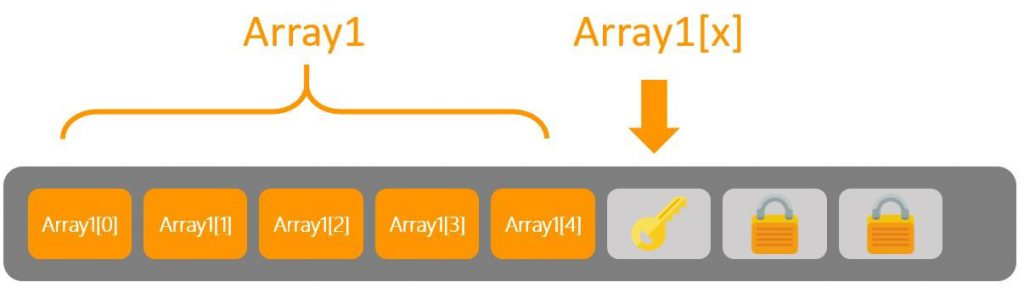
\includegraphics[scale=.3]{arraySpectre}
					\caption{recupero del valore al di fuori di \emph{array1}}
					\label{fig:array}
				\end{center}
			\end{figure}
			
			Per completare l'attacco, l'attaccante non deve fare altro che rilevare questo cambiamento nello stato della cache per recuperare il byte segreto \emph{k}.
			
			Nel caso più semplice, quello cioè in cui l'attaccante ha accesso diretto ad \emph{array2}, egli non dovrà fare altro che provare  a leggere tutte le posizioni di \arr{array2}{n*256} per tutti i valori di $n \in (0\dots255)$. Solamente uno di questi sarà presente in cache (quello per \emph{n} = \emph{k}) e verrà restituito velocemente mentre tutti gli altri verranno restituiti in tempi molto lunghi. Prendendo l'unico valore restituito in tempo breve, l'attaccante avrà trovato il byte segreto \emph{k}.
			
			Questo attacco può ovviamente essere eseguito un numero indeterminato di volte e può portare alla completa lettura della memoria della vittima un byte alla volta.
			
	\section{Le contromisure}
		Come detto all'inizio del capitolo, al momento attuale non sono state rilasciate patch a livello di hardware o di microprogrammazione del processore in grado di risolvere completamente il problema.
		
		La soluzione più ovvia è quella di non permettere l'esecuzione speculativa tout court ma questa scelta andrebbe ad impattare eccessivamente sulle prestazioni. L'idea è quella di cercare di impedire l'esecuzione speculativa su parti di codice compromettenti.
		
		In questa direzione, sia Intel che AMD, nei loro white papers \cite{AMD2018speculation,intel2018speculative}, suggeriscono alcune regole di programmazione per difendersi da questi attacchi.
		
		\subsection*{Serializzare gli accessi alla memoria}
		
		La prima regola è quella di serializzare gli accessi alla memoria tramite l'utilizzo dell'istruzione \emph{lfence()}\index{Lfence()}. Questa è un tipo di istruzione di \emph{barriera} che forza il processore o il compilatore ad una esecuzione ordinata delle operazioni di memoria richieste immediatamente prima ed immediatamente dopo la barriera. Tipicamente questo fa sì che sia garantito che l'istruzione che segue la barriera non venga eseguita prima di quella che la precede. A titolo di esempio, analizziamo il \cref{list:difendere}.
		
		\begin{lstlisting}[caption={codice da difendere},label={list:difendere}]
			if (user_value >= LIMIT) {
				return ERROR;
			} 
			x = table[user_value]; 
			node = entry[x];
		\end{lstlisting}
		
		In questo caso, la riga $4$ può essere eseguita speculativamente con il valore \emph{user\_value} fornito dall'attaccante mentre si attende il risultato del controllo presente alla riga $1$, ritardato perché il valore di \emph{LIMIT} non è presente in cache. 
		
		L'istruzione \emph{lfence()} alla riga $4$ del \cref{list:lfence} scongiura questa eventualità impedendo l'accesso alla memoria prima che sia terminato l'accesso precedente.
		
		\begin{lstlisting}[caption={utilizzo di lfence},label={list:lfence}]
		if (user_value >= LIMIT) {
			return ERROR;
		} 
		lfence(); 
		x = table[user_value]; 
		node = entry[x];
		\end{lstlisting} 
		
		Questa soluzione sicuramente risolve il problema ma ha due grossi difetti; deve essere inserita manualmente a livello di programmazione e porta una perdita di prestazioni notevole\cite{AMD2018speculation}.
		
		Microsoft implementa nel proprio compilatore una rilevazione automatica del codice vulnerabile agli attacchi di tipo SPECTRE ed inserisce tali barriere automaticamente. Purtroppo la blacklist di questo strumento comprende solamente le situazioni più comuni e maggiormente utilizzate. Kocher infatti dimostra che tale analisi automatica non rileva molte sezioni di codice vulnerabile\cite{kocher2018mitigation}.
		
		\subsection*{Utilizzare variabili "volatile"}
		
		Un'altra possibile contromisura può essere quella di utilizzare variabili dichiarate \emph{volatile} come nel \cref{cod:volatile}:
		
		\begin{lstlisting}[caption={utilizzo di variabili dichiarate volatile},label={cod:volatile}]
		volatile int user_value;
		/*
		* some untrusted operations 
		* to get the value of user_value
		*/
		if (user_value >= LIMIT) {
		return ERROR;
		} 
		x = table[user_value]; 
		node = entry[x];
		\end{lstlisting}
		
		L'attributo \emph{volatile} vieta al processore di cercare in cache il valore di variabili così dichiarate, bensì lo costringe a recuperarlo sempre dalla memoria principale, evitando che il compilatore esegua qualunque tipo di ottimizzazione di istruzioni contenenti tali variabili.
				
		Ovviamente anche questo metodo risolve il problema, ma come per il precedente influisce negativamente sulle prestazioni in quanto ogni volta che la variabile \emph{user\_value} viene utilizzata (anche in altri punti del programma) si dovrà sempre aspettare il suo recupero dalla memoria principale.
		
		\subsection*{Forzare le variabili entro i limiti}
		
		Questa ultima soluzione prevede di accertarsi che il valore di \emph{user\_value}, quando viene usato come indice, non vada mai a superare la dimensione del nostro array. Per ottenere questa certezza si può utilizzare l'operatore di modulo come nel \cref{list:limiti}:
		
		\begin{lstlisting}[caption={rispetto dei limiti forzato},label={list:limiti}]
		if (user_value >= LIMIT) {
		return ERROR;
		}
		x = table[user_value % LIMIT]; 
		node = entry[x];
		\end{lstlisting}
		
		In questo caso le situazioni possibili sono due:
		
		\begin{enumerate}
			\item \emph{user\_value} è minore di \emph{LIMIT} e quindi \emph{user\_value \% LIMIT} non cambia valore.
			\item \emph{user\_value} non è minore di \emph{LIMIT} ma \emph{user\_value \% LIMIT} lo riporta entro i limiti e non può essere utilizzato per leggere memoria esterna all'array.
		\end{enumerate}
	
		Come le precedenti, anche questa soluzione funziona, ma comporta un calo delle prestazioni dovuto al fatto che se la variabile \emph{LIMIT} non è in cache al momento del controllo, non lo sarà neanche quando verrà eseguita speculativamente l'istruzione della riga $4$ che quindi dovrà comunque aspettare il valore corretto. 
%\chapter{SPARK}
	In questo capitolo verrà analizzato \ac{SPARK}\index{SPARK}, il nostro attacco basato sul progetto SPECTRE capace di recuperare chiavi (o più in generale "segreti") evitando il controllo della password.
	
	\section{Scenario}
		Immaginiamo di partire dalla funzione attaccata da SPECTRE (\cref{list:vulnerabile}). Nello scenario più semplice si può pensare che \texttt{array1} (che d'ora in poi chiameremo \texttt{secret}) contenga delle chiavi predefinite assegnate ad ogni utente. Queste chiavi vengono utilizzate come indici  per accedere ad \texttt{array2}, che contiene le informazioni riservate di tutti gli utenti (ad esempio il saldo del conto corrente). Data la riservatezza di queste informazioni, l'accesso a questo array è protetto da una password. 
		
		L'utente \emph{x} che vorrà consultare i propri dati dovrà autenticarsi inserendo il proprio \texttt{userID} ed una password (salvata insieme alle password degli altri utenti nell'array \texttt{passwordDigest}). In caso di esito positivo del controllo, si utilizzerà il valore contenuto in \arr{secret}{userID} come indice di \texttt{array2} per andare a recuperare il dato sensibile riguardante x. In caso di esito negativo verrà ovviamente negato l'accesso ai dati.
		
		Tale funzione potrebbe essere implementata dal \cref{list:spark}:
		\codice{26}{30}{funzione attaccata da SPARK}{list:spark}
		
		Supponiamo adesso che l'attaccante abbia accesso ad \texttt{array2} (come supposto anche dall'attacco SPECTRE), ma che non abbia accesso all'array \texttt{secret} ed ovviamente neanche all'array delle password. L'obiettivo del nostro attacco è quello di ricavare, per un utente casuale \emph{x}, il relativo \arr{secret}{userID}, per poter successivamente avere accesso all'informazione riservata, il tutto senza conoscere la password.
		
		La precisione del risultato ottenuto dipende molto dal processore e dal tipo di dati utilizzato per rappresentare i diversi valori. Nella nostra implementazione abbiamo utilizzato il tipo primitivo \texttt{int} (dimensione 32 bit); questo, in una cache con dimensione delle line pari a $512$ bit (un valore considerato standard nei processori più moderni) non ci permette di recuperare esattamente \arr{secret}{x} (\cref{fig:lineSize}), tuttavia ci consente di localizzarlo in un intervallo di ampiezza $\delta$ con: $$\delta = \frac{\text{dimensione di una line}}{\text{dimensione del tipo di dato}} = \frac{512}{32} = 16.$$
		
		\begin{figure}
			\begin{center}
				
\includegraphics[width=.8\textwidth]{lineSize}
				\caption{contenuto di una cache line nel nostro setup}
				\label{fig:lineSize}
			\end{center}
		\end{figure}
		
		\section{L'attacco}
			Prima di analizzare l'effettiva implementazione, vediamo l'idea generale dell'attacco, che può essere schematizzato in quattro punti:
			
			\begin{enumerate}
				\item Il \ac{BP} viene addestrato richiamando la funzione vittima per tre volte con uno \texttt{userID} e la relativa password corretta. Per addestrare il BP, all'attaccante basterà semplicemente autenticarsi con i propri dati.
				\item Viene eseguito il \emph{flush} dalla cache di tutti i dati relativi ad \texttt{array2} e \texttt{passwordDigest}. Ricordiamo che l'istruzione \texttt{clflush} non richiede alcun privilegio per essere eseguita.
				\item Viene richiamata la funzione vittima con lo \texttt{userID} di cui vogliamo scoprire il segreto (che nel codice chiameremo \texttt{userUnderAttack}) ed una password casuale.
				\item Viene calcolato il tempo necessario ad accedere ad alcune posizioni di \texttt{array2}. Considerato che, data l'esecuzione speculativa dovuta alla chiamata precedente, l'unico dato relativo ad \texttt{array2} presente in cache in questo momento è \emph{y} = \arrdoppio{array2}{secret}{userUnderAttack}, otterremo un tempo basso solamente per una posizione presente nella stessa line che contiene \emph{y}. Per tutte le altre invece sarà alto in quanto il dato dovrà essere recuperato dalla memoria principale.
			\end{enumerate}
		
			Questo attacco sfrutta l'esecuzione speculativa del processore sul controllo della password. Infatti, avendo eseguito il \emph{flush} di \texttt{passwordDigest} al punto due, \emph{z} = \arr{passwordDigest}{userUnderAttack} non sarà presente in cache al momento del controllo al punto tre. Nell'attesa del suo recupero dalla memoria principale, il \ac{BP} eseguirà il ramo then della computazione a causa dell'addestramento ottenuto al punto uno. Il valore di \emph{y} verrà quindi prelevato dalla memoria e messo nella cache. Quando sarà disponibile \emph{z}, il controllo fallirà e non verrà permesso l'accesso ai dati, ma \emph{y} resterà in cache. A questo punto, accedendo a varie posizioni di \texttt{array2}, l'unica ad avere un tempo di accesso veloce sarà quella che ci dirà quale line contiene il segreto. La scelta delle posizioni da accedere e il calcolo del range viene spiegato più dettagliatamente nella prossima sezione.
			
			\subsection{Implementazione}
				Passiamo adesso all'analisi vera e propria del nostro programma che implementa l'attacco.
				
				\subsubsection{Inizializzazione}
				\codspark{1}{18}{inizializzazione}
				
				Nella primissima parte vengono semplicemente caricate le librerie necessarie alla compilazione, viene definito il numero di utenti (tremila), vengono creati i tre array principali (\texttt{secret}, \texttt{array2} e \texttt{passwordDigest}) e viene definita la funzione vittima, esattamente la stessa proposta nello scenario.
				
 				La libreria \texttt{x86intrin} fornisce le istruzioni \texttt{rdtscp} e \texttt{\_\_mm\_clflush} necessarie al calcolo dei tempi di hit e al flush della cache. In particolare l'istruzione \texttt{\_\_mm\_clflush} prende come argomento un indirizzo di memoria ed invalida, su tutti i livelli della cache, tutte le line che contengono quell'indirizzo.
				
				I tre array "utili" sono separati da altri array \texttt{unused} per essere sicuri che vengano distanziati in memoria. Questo fa sì che non si sovrappongano all'interno di una stessa line.
				
				\subsubsection{Main - definizione parametri}
				\codspark{19}{39}{main - definizione parametri}
				
				In questa parte vengono definiti i parametri che verranno utilizzati nel resto del programma:
				
				\begin{itemize}
					\item \texttt{CACHELINE}: la dimensione in bit di una singola cache line. Come già detto, questa dimensione è ormai standardizzata a $512$ bit su tutti i processori moderni.
					
					\item \texttt{blocks}: la dimensione in bit di un singolo elemento dell'array. In questo caso 32 bit.
					
					\item \texttt{delta}: il numero di elementi dell'array contenuti in una cache line.
					
					\item \texttt{class}: il numero di posizioni da controllare per coprire tutto \texttt{array2} con uno step pari a $\delta$. Questo valore fornisce anche il numero di line occupate in cache da \texttt{array2}.
					
					\item \texttt{numberOfRuns}: il numero di volte che viene eseguito l'attacco per ogni esperimento.
					
					\item \texttt{numberOfTests}: il numero di esperimenti che vengono eseguiti.
					
					\item \texttt{cacheHitThreshold}: la soglia entro la quale il tempo calcolato viene considerato una cache hit. Sperimentalmente questo valore si aggira tra i trenta e i quaranta cicli di clock, ma dipende dalla latenza della particolare cache attaccata.
					
					\item \texttt{precisionLoss}: con questo valore si regola la precisione che si vuole ottenere. Se lasciato a zero verrà restituito un intervallo di ampiezza $\delta$ che dovrebbe contenere il segreto. A volte però può succedere che l'intervallo calcolato non contenga il segreto a causa di interferenze con altri processi che utilizzano il processore, o a causa di un diverso allineamento delle cache. Aumentando questo valore si aumenta l'ampiezza dell'intervallo proporzionalmente a $\delta$, perdendo un po' in localizzazione, ma guadagnando in correttezza dell'intervallo (questo, insieme a \texttt{numberOfRuns}, \texttt{numberOfTests} e \texttt{cacheHitThreshold} sono i quattro parametri richiesti all'avvio del programma).		
								
					\item \texttt{results}: l'array nel quale verrà salvato il numero di hit rilevate per ogni line di cache.
					
					\item \texttt{ok}, \texttt{error} e \texttt{no-hit}: tre contatori utilizzati rispettivamente per sapere quante volte il programma restituisce l'intervallo che contiene il segreto, quante volte lo restituisce sbagliato e quante volte non rileva nessun cache hit.
					
					\item \texttt{timeReg}, \texttt{time1} e \texttt{time2}: le tre variabili per calcolare i tempi di accesso alle posizioni di \texttt{array2}.
				\end{itemize}			
				Dopo aver definito tutti i parametri, si procede con l'inizializzazione del generatore \texttt{srand()} di numeri casuali.
				
				\subsubsection{Main - inizializzazione dell'esperimento}
				\codspark{40}{51}{main - inizializzazione dell'esperimento}
				
				All'inizio di ogni test viene scelto casualmente lo \texttt{userUnderAttack} e vengono inizializzati casualmente i tre array principali \texttt{passwordDigest}, \texttt{array2} e \texttt{secret}. Successivamente si sceglie una password sicuramente sbagliata ed infine si prepara l'array \texttt{results} al conteggio delle hit settandolo a zero.
				
				\subsubsection{Main - l'attacco}
				\codspark{52}{71}{main - l'attacco}
				
				Come descritto nello scenario, l'attacco si divide in quattro parti. Nella prima parte viene addestrato il \ac{BP} ad eseguire speculativamente il ramo then della funzione vittima, richiamandola per tre volte con \texttt{userID} e password corretta.
				
				Successivamente si esegue il flush dalla cache di tutte le posizioni degli array \texttt{array2} e \texttt{passwordDigest}.
				
				Prima di richiamare la funzione vittima facciamo eseguire l'istruzione \texttt{\_mm\_lfence}. Tale istruzione è una barriera sulla memoria che non permette l'esecuzione delle istruzioni successive prima che siano terminate tutte le scritture in memoria delle istruzioni precedenti. Questo evita ad esempio che l'istruzione a riga $90$ venga eseguita prima del flush di \texttt{array2} a causa di un riordinamento del codice. Se accadesse questo, il risultato del calcolo del tempo di accesso sarebbe ovviamente falsato.
				
				Terminato il flush della cache, viene richiamata la funzione vittima e vengono calcolati i tempi di accesso alle varie posizioni di \texttt{array2}. Come si può notare, non si effettua l'accesso a tutte le posizioni di \texttt{array2} ma si procede con un passo $\delta$ visto che una qualunque delle $\delta$ posizioni all'interno della line che contiene il segreto restituirà comunque una hit.
				
				Con un'altra \texttt{\_mm\_lfence} ci assicuriamo che il tempo venga effettivamente salvato in \texttt{time2} ed effettuiamo il controllo. Se il risultato del calcolo del tempo di accesso è minore della soglia che abbiamo impostato, aumentiamo di uno nell'array \texttt{results} il valore  contenuto all'indice che stiamo analizzando.
				
				\subsubsection{Main - i risultati}
				\codspark{72}{105}{main - i risultati}
				
				\begin{figure}[b]
					\begin{center}
						
\includegraphics[width=\textwidth]{range}
						\caption{calcolo del range}
						\label{fig:range}
					\end{center}
				\end{figure}
				
				Nell'ultima parte del programma viene cercato l'indice \texttt{index} con il valore più alto nell'array \texttt{results}. Questo indice rappresenta la porzione di \texttt{array2} che dovrebbe contenere il segreto. Da questo indice viene calcolato il range da restituire (\cref{fig:range}) limitato in basso da $0$ ed in alto da \texttt{SIZE} che non è altro che: $$((index - precisionLoss) * \delta\ ,\ (index + 1 + precisionLoss) * \delta).$$ Il risultato così ottenuto viene infine comparato con \arr{secret}{userUnderAttack} e viene stabilito il risultato dell'attacco:
				
				\begin{itemize}
					\item \texttt{OK} - se il segreto ricade nel range calcolato.
					\item \texttt{ERROR} - se il segreto non ricade nel range calcolato.
					\item \texttt{NO-HIT} - se non si è rilevata alcuna hit.
				\end{itemize}
				
				Come ultima cosa viene visualizzato sullo schermo un resoconto dei risultati ottenuti. Nella \cref{fig:schermata} si può vedere la schermata del programma.
				
				\begin{figure}
					\begin{center}
						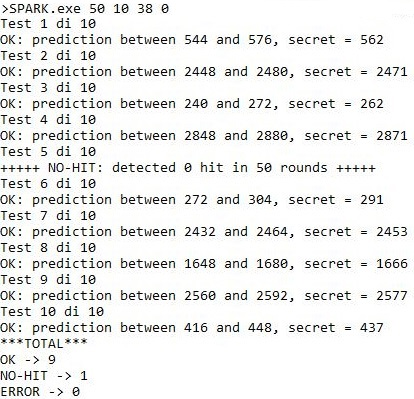
\includegraphics[width=.6\textwidth]{risultati}
						\caption[schermata di SPARK]{schermata del programma lanciato con i parametri $50,100,38,0$}
						\label{fig:schermata}
					\end{center}
				\end{figure}
			
			\subsection{Prove sperimentali}
				Abbiamo testato il programma su un notebook SAMSUNG-R$580$ che monta un processore INTEL CORE i$3$-$330$M a $2.13$\gigahertz e su un computer desktop equipaggiato con un processore i$7$-$4700$MQ a $2.40$\gigahertz. Di seguito i risultati ottenuti con ognuno dei due.
				
				\subsubsection*{INTEL CORE i$3$-$330$M} 
				
					Questo processore dispone di tre livelli di cache così suddivisi:
					
					\begin{itemize}
						\item [L$1$ -] $2$ x $64$ \kilobyte \ divise in 
						\begin{itemize}
							\item  $2$ x $32$ \kilobyte \ $4$-way associative cache per i dati
							\item  $2$ x $32$ \kilobyte \ $8$-way associative cache per le istruzioni
						\end{itemize}
						\item[L$2$ -] $2$ x $256$ \kilobyte \ $8$-way associative cache
						\item[L$3$ -] $3$ \megabyte \ $12$-way associative cache condivisa dai due core
					\end{itemize}
				
					\begin{figure}
						\begin{center}
							
\includegraphics[width=\textwidth]{risultatiTab}
							\caption{risultati ottenuti sul processore i$3$-$330$M}
							\label{fig:risultati}
						\end{center}
					\end{figure}
				
					Abbiamo effettuato dieci sessioni di esperimenti (i cui risultati sono visibili in \cref{fig:risultati}), ognuna composta da tremila test suddivisi in:
					
					\begin{itemize}
						\item mille in cui vengono eseguiti venti run ogni test
						\item mille in cui vengono eseguiti cinquanta run ogni test
						\item mille in cui vengono eseguiti cento run ogni test.
					\end{itemize}
					
					Come è normale aspettarsi, maggiore è il numero di round effettuato per ogni test, maggiore è la precisione che si ottiene. Nei nostri esperimenti si passa infatti da una media di successi ottenuti del $79.8\%$ con venti round a $98.2\%$ con cento round. Ovviamente, aumentando il numero di round, aumenta il tempo di esecuzione che nei due casi precedenti passa, per ogni test, da meno di un secondo a circa cinque secondi.
					
				\subsubsection*{INTEL CORE i$7$-$4700$MQ} 
				
					Anche questo processore dispone di tre livelli di cache così suddivisi: 
					
					\begin{itemize}
						\item [L$1$ -] $4$ x $64$ \kilobyte \ divise in 
						\begin{itemize}
							\item  $4$ x $32$ \kilobyte \ $8$-way associative cache per i dati
							\item  $4$ x $32$ \kilobyte \ $8$-way associative cache per le istruzioni
						\end{itemize}
						\item[L$2$ -] $4$ x $256$ \kilobyte \ $8$-way associative cache
						\item[L$3$ -] $6$ \megabyte \ $12$-way associative cache condivisa dai quattro core
					\end{itemize}
					
					\begin{figure}
						\begin{center}
							
\includegraphics[width=\textwidth]{risultatiTab2}
							\caption{risultati ottenuti sul processore i$7$-$4700$MQ}
							\label{fig:risultati2}
						\end{center}
					\end{figure}
					
					Anche in questo caso abbiamo effettuato dieci sessioni di esperimenti (i cui risultati sono visibili in \cref{fig:risultati2}), esattamente identiche alle precedenti.
					
					Le indicazioni ottenute sono in linea con i test eseguiti sull'altro processore con una precisione che aumenta all'aumentare del numero di round. In questo caso si parte infatti da una media di successi ottenuti del $95.3\%$ con venti round fino ad arrivare al $99.2\%$ con cento round. Utilizzando un processore con prestazioni migliori, i tempi di esecuzione si sono sensibilmente abbassati: si passa da circa $0.4$ secondi a test se effettuati con venti round a $2$ secondi a test se effettuati con cento round (circa il doppio più veloce del precedente).
					
					Anche il maggior numero di errori è molto probabilmente dovuto alle migliori prestazioni del processore. Trattandosi di un computer general purpose, equipaggiato con Windows $10$ come sistema operativo, nel tempo di esecuzione del programma altri processi possono interagire con la cache creando così delle false hit. 
					
					Sarebbe interessante eseguire questi esperimenti su macchine dedicate esclusivamente all'esecuzione di questo programma per capire quanto l'influenza di processi esterni possa interferire con l'esecuzione di SPARK. 
					
%\chapter{Conclusioni}
	Durante lo svolgimento di questa tesi ci è risultato evidente l'attuale fermento presente nell'ambiente scientifico e industriale riguardo agli attacchi di tipo side-channel, in particolar modo su quelli della famiglia SPECTRE. Vengono pubblicati continuamente articoli accademici che spiegano nuovi attacchi o varianti di quelli già conosciuti e, di conseguenza, vengono rilasciate dalle varie case costruttrici di processori nuove contromisure. Più in generale, vengono diffuse in rete un numero impressionante di informazioni su questo tema.
	
	\`{E} proprio di pochi giorni fa (agosto 2018) l'aggiunta di una nuova variante agli attacchi della famiglia SPECTRE denominata \emph{FORESHADOW}\cite{bulck2018foreshadow}.
	
	L'idea che ci siamo fatti è che sia stato appena aperto un vaso di Pandora che sta mettendo in crisi la sicurezza di milioni di macchine in tutto il mondo. Le case costruttrici (Intel soprattutto) stanno cercando di mitigare questi attacchi sui vecchi processori con aggiornamenti al microcode e, in collaborazione con i produttori dei principali sistemi operativi, con aggiornamenti ai kernel. Sui processori di nuova generazione ci sarà bisogno di una riprogettazione sostanziosa per evitare, fin dal primo momento, di ritrovarsi ancora in questo tipo di situazioni. Fortunatamente la cultura della sicurezza, che fino a poco tempo fa veniva ritenuta un male necessario, sta prendendo piede anche fra i non addetti ai lavori. 
	
	\`{E} appurato che la maggior parte degli attacchi informatici sfrutta falle dovute alla ricerca di miglioramento di prestazioni a discapito della robustezza del programma. Trovare il giusto bilanciamento tra prestazioni e sicurezza è sicuramente molto difficile, ma se vogliamo evitare che disastri del genere si verifichino di nuovo, dovremo privilegiare sempre di più la seconda, eventualmente a discapito della prima.
	
	\section{Sviluppi futuri}
		SPARK può essere considerato un \ac{PoC} che mette in luce la possibilità di accedere a dati protetti da password. Partendo dalla sua attuale implementazione, potrebbe essere sviluppato applicandolo a funzioni crittografiche nei sistemi reali. 
		
		Un'ulteriore direzione di sviluppo può essere quella di rendere remoto l'attacco. Attualmente SPARK deve essere eseguito sulla macchina della vittima e questo limita sicuramente le sue capacità. Riuscire ad ottenere da remoto gli stessi dati ottenuti con una esecuzione locale sarebbe un grande passo avanti. Per far questo bisognerebbe pensare ad un approccio statistico che riesca a filtrare il rumore dovuto ai tempi di trasmissione delle informazioni.
		
		Infine, si potrebbe cercare di renderlo "universale". Al momento infatti SPARK funziona solamente su processori con architettura $x86$. Sarebbe interessante riuscire ad implementarne una versione in grado di attaccare altre architetture come ad esempio \ac{ARM}, largamente utilizzata nel mondo mobile o embedded.
	
	
	

%-----------------APPENDICI------------------------------------

%\appendix
%\chapter{OWASP Mobile Top 10 risks}

	Si riporta la lista "Mobile top $10$ $2016$"\cite{OWASPtop10} stilata da OWASP Foundation:
	
	\begin{itemize}
		\item \textbf{M1 - Improper Platform Usage}; This category covers misuse of a platform feature or failure to use platform security controls. It might include Android intents, platform permissions, misuse of TouchID, the Keychain, or some other security control that is part of the mobile operating system. There are several ways that mobile apps can experience this risk.
		\item \textbf{M2 - Insecure Data Storage}; This new category is a combination of M2 + M4 from Mobile Top Ten 2014. This covers insecure data storage and unintended data leakage.
		\item \textbf{M3 - Insecure Communication}; This covers poor handshaking, incorrect SSL versions, weak negotiation, cleartext communication of sensitive assets, etc.
		\item \textbf{M4 - Insecure Authentication}; This category captures notions of authenticating the end user or bad session management. This can include:
		\begin{itemize}
			\item Failing to identify the user at all when that should be required
			\item Failure to maintain the user's identity when it is required
			\item Weaknesses in session management
		\end{itemize}		
		\item \textbf{M5 - Insufficient Cryptography}; The code applies cryptography to a sensitive information asset. However, the cryptography is insufficient in some way. Note that anything and everything related to TLS or SSL goes in M3. Also, if the app fails to use cryptography at all when it should, that probably belongs in M2. This category is for issues where cryptography was attempted, but it wasn't done correctly.
		\item \textbf{M6 - Insecure Authorization}; This is a category to capture any failures in authorization (e.g., authorization decisions in the client side, forced browsing, etc.). It is distinct from authentication issues (e.g., device enrolment, user identification, etc.). If the app does not authenticate users at all in a situation where it should (e.g., granting anonymous access to some resource or service when authenticated and authorized access is required), then that is an authentication failure not an authorization failure.
		\item \textbf{M7 - Client Code Quality}; This was the "Security Decisions Via Untrusted Inputs", one of our lesser-used categories. This would be the catch-all for code-level implementation problems in the mobile client. That's distinct from server-side coding mistakes. This would capture things like buffer overflows, format string vulnerabilities, and various other code-level mistakes where the solution is to rewrite some code that's running on the mobile device.
		\item \textbf{M8 - Code Tampering}; This category covers binary patching, local resource modification, method hooking, method swizzling, and dynamic memory modification. Once the application is delivered to the mobile device, the code and data resources are resident there. An attacker can either directly modify the code, change the contents of memory dynamically, change or replace the system APIs that the application uses, or modify the application's data and resources. This can provide the attacker a direct method of subverting the intended use of the software for personal or monetary gain.
		\item \textbf{M9 - Reverse Engineering}; This category includes analysis of the final core binary to determine its source code, libraries, algorithms, and other assets. Software such as IDA Pro, Hopper, otool, and other binary inspection tools give the attacker insight into the inner workings of the application. This may be used to exploit other nascent vulnerabilities in the application, as well as revealing information about back end servers, cryptographic constants and ciphers, and intellectual property.
		\item \textbf{M10 - Extraneous Functionality}; Often, developers include hidden backdoor functionality or other internal development security controls that are not intended to be released into a production environment. For example, a developer may accidentally include a password as a comment in a hybrid app. Another example includes disabling of 2-factor authentication during testing.
	\end{itemize} 
%\chapter{SPARK - Codice completo e commentato}

	\lstinputlisting[language={C},caption={SPARK - codice completo e commentato}]{"D:/UNIFI/Magistrale/Tesi/spectre/primeProbe/spark.c"}
	
	\cleardoublepage
	\thispagestyle{empty}
	\begin{figure}
		\begin{center}
			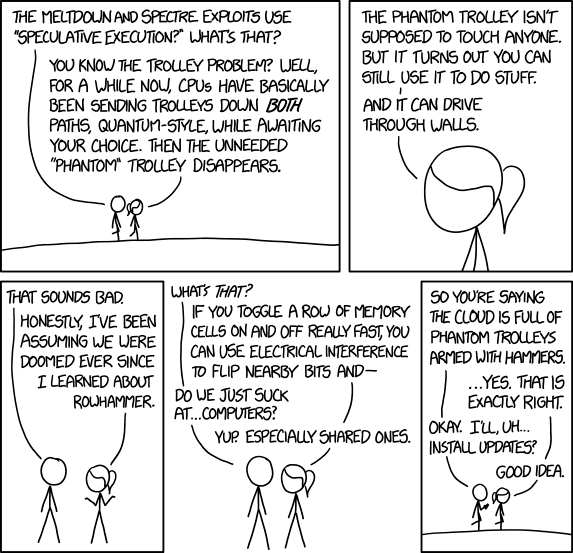
\includegraphics[width=\textwidth]{xkcd}
			\caption[XKCD 1938 - SPECTRE e Meltdown]{\href{https://xkcd.com/1938/}{XKCD 1938 - SPECTRE e Meltdown}}
		\end{center}
	\end{figure}

%-----------------BIBLIOGRAFIA---------------------------------

%\bibliography{bib/bibliografia}
%\bibliographystyle{unsrt}

%-----------------INDICI---------------------------------------

\addcontentsline{toc}{chapter}{Acronimi}

\chapter*{Acronimi}
	\begin{acronym}[CAGD]
		\acro{AES}{Advanced Encryption Standard}
		\acro{ARM}{Advanced RISC Machine}
		\acro{BP}{Branch Predictor}
		\acro{CNES}{Centre National d’Etudes Spatiales}
		\acro{CRT}{Chinese Remainder Theorem}
		\acro{CVE}{Common Vulnerabilities and Exposures}
		\acro{DBA}{Differential Behavior Analysis}
		\acro{DES}{Data Encryption Standard}
		\acro{DFA}{Differential Fault Analysis}
		\acro{DFIA}{Differential Fault Intensity Analysis}
		\acro{DH}{Diffie-Hellman}
		\acro{DPA}{Differential Power Analysis}
		\acro{DSA}{Digital Signature Algorithm}
		\acro{DSS}{Digital Signature Standard}
		\acro{FBA}{Fault Behavior Analysis}
		\acro{FIPS}{Federal Information Processing Standards}
		\acro{FSA}{Fault Sensitivity Analysis}
		\acro{GPS}{Global Positioning System}
		\acro{HTTPS}{HyperText Transfer Protocol over Secure Socket Layer}
		\acro{LED}{Light Emitting Diode}
		\acro{LLC}{Last Level Cache}
		\acro{NATO}{North Atlantic Treaty Organization}
		\acro{NCSCD4}{National Communications Security Committee Directive 4}
		\acro{NIST}{National Institute of Standards and Technology}
		\acro{PICA}{Picosecond Imaging Circuit Analysis}
		\acro{PoC}{Proof of Concept}
		\acro{QIF}{Quantitative Information-flow Analysis}
		\acro{SEA}{Safe-Error Attacks}
		\acro{SPA}{Simple Power Analysis}
		\acro{SPARK}{Spectre-based Password-avoiding Attack to Retrieve Keys}
		\acro{TEMPEST}{Transient Electromagnetic Pulse Emanation STandard}
		\acro{TOR}{The Onion Router}
	  	\acro{USB}{Universal Serial Bus}
	\end{acronym}
\printindex
\end{document}